\documentclass[10pt, a4paper,english,spanish]{article}
%\documentclass[10pt,a4paper]{article}
\usepackage[utf8]{inputenc} % para poder usar tildes en archivos UTF-8
\usepackage[spanish]{babel} % para que comandos como \today den el resultado en castellano
\usepackage[conEntregas]{caratula}
\usepackage{fullpage} %small margins
\usepackage[parfill]{parskip} %genera saltos entre parrafos
\usepackage{color}
\definecolor{gray}{gray}{0.35}
\usepackage{listings}
\usepackage{enumitem}
\usepackage{amsmath} %big brackets
\usepackage[pdftex]{graphicx}
\lstset{
    numbers=left,
    breaklines=true,
    tabsize=2,
    basicstyle=\ttfamily\color{gray},
}
\setlength{\parindent}{8pt}
\usepackage{mathtools}
\usepackage[margin=50pt]{geometry}
\usepackage{amsfonts}
\usepackage{flafter}
\usepackage{multicol}
\begin{document}

\materia{Algoritmos y Estructuras de Datos III}
\submateria{Trabajo Práctico Nro. 3}
\titulo{Heurísticas y Metaheurísticas}
\fecha{\today}
\integrante{Pablo Gomez}{156/13}{mago-1986@hotmail.com}
\integrante{Lucia Parral}{162/13}{luciaparral@gmail.com}
\integrante{Emanuel Lamela}{21/13}{emanuel93\_13@hotmail.com}
\integrante{Petr Romachov}{412/13}{promachov@gmail.com}
\maketitle
\newpage

\tableofcontents

\newpage
% Comienzo Ejercicio 1
\documentclass[10pt,a4paper]{article}
\usepackage[utf8]{inputenc} % para poder usar tildes en archivos UTF-8
\usepackage[spanish]{babel} % para que comandos como \today den el resultado en castellano
\usepackage{fullpage} %small margins
\usepackage[parfill]{parskip} %genera saltos entre parrafos
\usepackage{color}
\definecolor{gray}{gray}{0.35}
\usepackage{listings}
\usepackage{enumitem}
\usepackage{amsmath} %big brackets
\lstset{
    numbers=left,
    breaklines=true,
    tabsize=2,
    basicstyle=\ttfamily\color{gray},
}
\setlength{\parindent}{8pt}
\usepackage{mathtools}
\usepackage[margin=50pt]{geometry}
\usepackage{amsfonts}
\usepackage{flafter}
\newcommand{\tab}[1]{\hspace{.1\textwidth}\rlap{#1}}
\usepackage{graphicx}
\begin{document}

\section{Ejercicio 1}
\subsection{Introducción}
\indent \subsubsection{Contexto}
Estamos en el desarrollo de un sitio web de compra de pasajes aéreos, conocido como aterrizar.com. Nuestro sitio ofrece, entre sus otras opciones de búsqueda, una en particular que es innovadora, perfecta para impacientes/viajeros apurados, la cual consiste en que detallando el punto de origen y el punto de destino, el sistema indicará al usuario el itinerario que llega lo antes posible al destino seleccionado; todo esto el sistema lo hará siempre y cuando exista un posible itinerario que conecte ambos puntos.
La solución provista puede utilizar la cantidad de tramos que sean necesarios, ya que su único objetivo es optimizar la fecha y hora de llegada a destino.
\indent \subsubsection{El problema a resolver}

Nos encontramos entonces frente al desafío de desarrollar un algoritmo que se encargue de dicho itinerario, es decir, que dados los puntos de origen y destino, A y B respectivamente, y una lista de vuelos disponibles, debemos devolver un itinerario tal que vaya desde A hasta B, de la manera rápida posible. Para eso podemos combinar todos los vuelos que hagan falta pasando por cualquier ciudad intermedia en el camino.
De cada vuelo de la lista de disponibles conocemos su origen y destino y las fechas y horas de partida y llegada.
El algoritmo debe devolver un itinerario factible, y para ello, deben cumplirse las siguientes condiciones:

\indent• El primer vuelo debe salir de A y el último vuelo debe terminar en B.\\
\indent• Si el itinerario usa más de un vuelo, la ciudad de llegada de cada vuelo debe coincidir con la ciudad de salida del vuelo siguiente.

Además, debe haber al menos 2 horas de diferencia entre la llegada de un vuelo y la partida del vuelo siguiente para los tiempos de embarque pertinentes entre un vuelo y otro.
\indent \subsubsection{Ejemplos}

\noindent \begin{enumerate}
\item
Ciudad de origen: Buenos Aires\\
Ciudad de destino: Jujuy\\
Cantidad de vuelos: 10\\

\begin{center}
	\begin{tabular}{| l | l | l | l |}
	\hline
	Ciudad De Origen & Ciudad Destino & Hora Salida & Hora Llegada\\ \hline
	Buenos Aires & La Pampa & 10 &	12\\
	Buenos Aires & Entre Ríos & 9 & 10 \\
	Buenos Aires & Formosa	&	11	& 13\\
	Formosa	& Córdoba	& 16 & 17  \\
	Entre Ríos & Jujuy	& 12 & 20\\
	Entre Ríos & La Rioja	&	13 & 15\\
	La Rioja & Tucuman	&	20 & 21\\
	Santiago del Estero & Jujuy &	20 & 22\\
	Santiago del Estero	& Catamarca & 23 & 24\\
	La Rioja & Santiago del Estero & 17&18\\
	\hline
	\end{tabular}
\end{center}


En este ejemplo hay dos itinerarios que llevan de la ciudad de origen, Buenos Aires a la de destino, Jujuy, cumpliendo que entre cada vuelo haya un mínimo de dos horas de diferencia entre la llegada de uno y el despege del siguiente:
\begin{itemize}
\item[•] (Buenos Aires - Entre Ríos) - (Entre Ríos - La Rioja) - (La Rioja - Santiago del Estero) - (Santiago del Estero - Jujuy) - \textbf{Horario de llegada: } 22hs

\item[•] (Buenos Aires - Entre Ríos) - (Entre Ríos - Jujuy) \textbf{Horario de llegada: } 20hs
\end{itemize}

Por lo tanto la solución es el segundo itinerario, ya que tiene un horario de llegada menor.\\

\item
Ciudad de origen: Buenos Aires\\
Ciudad de destino: Jujuy\\
Cantidad de vuelos: 10\\

\begin{center}
	\begin{tabular}{| l | l | l | l |}
	\hline
	Ciudad De Origen & Ciudad Destino & Hora Salida & Hora Llegada\\ \hline
	Buenos Aires & La Pampa & 10 &	12\\
	Buenos Aires & Entre Ríos & 9 & 10 \\
	Buenos Aires & Formosa	&	11	& 13\\
	Formosa	& Córdoba	& 16 & 17  \\
	Entre Ríos & Jujuy	& 11 & 20\\
	Entre Ríos & La Rioja	&	13 & 15\\
	La Rioja & Tucuman	&	20 & 21\\
	Santiago del Estero & Jujuy &	20 & 22\\
	Santiago del Estero	& Catamarca & 23 & 24\\
	La Rioja & Santiago del Estero & 17&18\\
	\hline
	\end{tabular}
\end{center}


En este ejemplo, se pierde el itinerario óptimo encontrado en el ejemplo anterior, ya que entre el primer vuelo (Buenos Aires - Entre Ríos) y el segundo (Entre Ríos - Jujuy) ya no hay un mínimo de 2 horas entre el horario de llegada de uno y el horario de partida del otro, por lo que nos queda una única solución, que es también óptima:

(Buenos Aires - Entre Ríos) - (Entre Ríos - La Rioja) - (La Rioja - Santiago del Estero) - (Santiago del Estero - Jujuy) - \textbf{Horario de llegada: } 22hs\\



\item
Ciudad de origen: Buenos Aires\\
Ciudad de destino: Jujuy\\
Cantidad de vuelos: 10\\

\begin{center}
	\begin{tabular}{| l | l | l | l |}
	\hline
	Ciudad De Origen & Ciudad Destino & Hora Salida & Hora Llegada\\ \hline
	Buenos Aires & La Pampa & 10 &	12\\
	Buenos Aires & Entre Ríos & 9 & 10 \\
	Buenos Aires & Formosa	&	11	& 13\\
	Misiones	& Córdoba	& 16 & 17  \\
	Corrientes & Jujuy	& 12 & 20\\
	Corrientes & La Rioja	&	13 & 15\\
	La Rioja & Tucuman	&	20 & 21\\
	Santiago del Estero & Jujuy &	20 & 22\\
	Santiago del Estero	& Catamarca & 23 & 24\\
	La Rioja & Santiago del Estero & 17&18\\
	\hline
	\end{tabular}
\end{center}

En este ejemplo, no hay ninguna silución, ya que si bien hay vuelos que salen desde la ciudad de origen Buenos Aires, no es posible realizar a partir del primer vuelo ninguna conexión para poder llegar a la ciudad de destino.\\


\item
Ciudad de origen: Buenos Aires\\
Ciudad de destino: Jujuy\\
Cantidad de vuelos: 10\\

\begin{center}
	\begin{tabular}{| l | l | l | l |}
	\hline
	Ciudad De Origen & Ciudad Destino & Hora Salida & Hora Llegada\\ \hline
	Buenos Aires & La Pampa & 10 &	12\\
	Buenos Aires & Entre Ríos & 9 & 10 \\
	Buenos Aires & Formosa	&	11	& 13\\
	Formosa	& Córdoba	& 16 & 17  \\
	Entre Ríos & Jujuy	& 12 & 20\\
	Entre Ríos & La Rioja	&	11 & 12\\
	La Pampa & Tucuman	&	14 & 15\\
	Tucumán & Jujuy &	17 & 20\\
	Santiago del Estero	& Catamarca & 23 & 24\\
	La Rioja & Santiago del Estero & 17&18\\
	\hline
	\end{tabular}
\end{center}
\newpage

En este ejemplo hay dos itinerarios que son solución óptima:

\begin{itemize}
\item[•] (Buenos Aires - Entre Ríos) - (Entre Ríos - La Rioja) \textbf{Horario de llegada: } 20hs

\item[•] (Buenos Aires - La Pampa) - (La Pampa - Tucumán) - (Tucumán - Jujuy) \textbf{Horario de llegada: } 20hs\\
\end{itemize}


\item
Ciudad de origen: Buenos Aires\\
Ciudad de destino: Jujuy\\
Cantidad de vuelos: 10\\

\begin{center}
	\begin{tabular}{| l | l | l | l |}
	\hline
	Ciudad De Origen & Ciudad Destino & Hora Salida & Hora Llegada\\ \hline
	Chubut & La Pampa & 10 &	12\\
	Río Negro & Entre Ríos & 9 & 10 \\
	Neuquén & Formosa	&	11	& 13\\
	Formosa	& Córdoba	& 16 & 17  \\
	Entre Ríos & Jujuy	& 12 & 20\\
	Entre Ríos & La Rioja	&	11 & 12\\
	La Pampa & Tucuman	&	14 & 15\\
	Tucumán & Jujuy &	17 & 20\\
	Santiago del Estero	& Catamarca & 23 & 24\\
	La Rioja & Santiago del Estero & 17&18\\
	\hline
	\end{tabular}
\end{center}

Ningún vuelo sale de la ciudad de Origen, por lo tanto, no hay solución.





\end{enumerate}

\newpage
\subsection{Desarrollo}


Para resolver el problema planteado, utilizamos la técnica de programación dinámica y un algoritmo top down, ya que presentaba las características necesarias para usarla, en tanto tiene subestructuras óptimas, es decir era posible dividir el problema en subproblemas más pequeños.\\

Por ejemplo, si quiero viajar de la ciudad A a la B de manera óptima, si el camino óptimo incluye ir de la ciudad X a B, y desde A es posible llegar a B, entonces el camino óptimo es el camino óptimo de A a X y de X a B.\\
.
Finalmente, al utilizar todas estas subsoluciones óptimas de viajes de cualquier ciudad a la ciudad de destino, se puede formar la solución al problema. Para esto, almacenaremos las soluciones ya calculadas para no tener que recalcularlas al momento de volver a necesitarlas.\\

Teniendo esto en mente, el algoritmo ideado para resolver el problema se basa principalmente en dos etapas:\\

\textbf{Preparación de los datos y almacenamiento en estructuras de datos:}


\begin{itemize}
\item A: Ciudad de origen
\item B: Ciudad objetivo
\item n: Cantidad de vuelos
\item Io: Ciudad origen del vuelo I
\item Id: Ciudad destino del vuelo I
\item Ip: Hora de partida del vuelo I
\item If: Hora de llegada del vuelo I
\item intCityMapping: diccionario\textless string,int\textgreater
\item salidas: vector\textless vector\textless Vuelo\textgreater\textgreater \\
\end{itemize}
\begin{lstlisting}
	salidas.reservarLugarPosiciones(n*2 + 2)
	Para i = 0 hasta n-1 hacer
			Si Io no esta definida en intCityMapping        O(log n)
				agregar	Io a intCityMapping                   O(log n)	
				agrandar en 1 el tamano del vector salidas    O(1) (reserved memory)
				
			Si Id no esta definida en intCityMapping        O(log n)
				agregar	Id a intCityMapping				            O(log n)	
				agrandar en 1 el tamano del vector salidas    O(1) (reserved memory)	
		
			IDciudadOrigen <- intCityMapping[Io]				    O(log n)
			IDciudadDestino <- intCityMapping[Id]				    O(log n)			
			
			Vuelo vuelo <- (IDciudadOrigen,IDciudadDestino,Ip,If,i+1)	  O(1)		
			salidas[IDciudadOrigen].agregarAtras(vuelo)     O(1) (reserved memory)
	Fin Para	
			
	Para j = 0 hasta salidas.size()-1 hacer
			ordenar(salidas[j])		O(x log x) (x = cantidad de vuelos que salen de j)
	Fin Para
\end{lstlisting}

Se mapean los vuelos pasados en el input, de modo de formar una matriz en la que para cada ciudad están los vuelos que salen de ella.\\
Luego, cada uno de los vuelos que parten de cada ciudad, los ordenaremos según su horario de salida.\\
A partir de este momento, los datos están almacenados en la forma necesaria para poder aplicar el algoritmo de mejor camino con la complejidad requerida.\\\\
\newpage	


\textbf{Cálculo del mejor itinerario:}\\

\begin{lstlisting}
vector<bool>  de cantidadDeCiudades posiciones, con todas inicializadas en bool
mejorCamino(int origen, int horaDeConsulta):
	revisadoHasta <- Infinit	
	
	Si(origen == ID representativo de ciudad B)
		cache[origen] <- (calculado, puedeLlegarAB, horaDeConsulta,horaDeConsulta)
		return cache[origen]
	Fin Si
	
	Si(cache[origen] tiene un calculo igual a horaDeConsulta)
		return cache[origen]	
	Sino
		revisadoHasta <- cache[origen].horaDeCalculo
	Fin Si
	
	Si(cache[origen] tiene un calculo a una hora menor)
	 	return Itinerario(calculado,hayOtroOptimo, Infinit, horaDeCalculo)
	Fin Si
	
	////////Variables
	itinerario <- Itinerario(calculado,noLlegahastaB,Infinit,horaDeConsulta)
	from <- 0
	esNecesarioSeguirRevisando <- true
	Si(vuelosDeSalida[origen].tam > 0)
		from <- customBinarySearch(hora, vuelosDeSalida[origen])
	
	//Ciclo
	para i = from  hasta  vuelosDeSalida[origen].tam-1 hacer
		vuelo := vuelosDeSalida[origen][i]

		Si(disponibles[vuelo.destino])
			Si(best[origen].calculado && revisadoHasta+2 <= vuelo.inicio)
					potencial = best[origen];
					esNecesarioSeguirRevisando <- false;
			Sino			
				disponibles[origen] <- false		//Apago la ciudad.
				recursivo <- mejorCamino(vuelo.destino, vuelo.fin);
			Fin Si
			
			Si(recursivo.puedeLlegarAB && recursivo.llegada < itinerario.llegada)
				itinerario<-(calculado,puedeLlegarAB,horaDeConsulta,recursivo.llegada)
			Fin Si
			
			Si(!esNecesarioSeguirRevisando)
				break
			Fin Si
			
		fin si
		
		disponibles[origen] <- true		//Activo la ciudad de nuevo
	fin para
	
	best[origen] = itinerario
	return best[origen]
fin mejorCamino 
\end{lstlisting}
\newpage

Llamaremos:
\begin{itemize}
\item Vuelo a la clase que contiene Origen (ciudad desde donde parte), Destino (ciudad a la cual se quiere llegar), hora de salida del vuelo y hora de llegada.
\item Ciuda\_Origen a la ciudad desde la cual se parte en la instancia pasada.
\item Ciuda\_Destino a la ciudad a la cual se quiere llegar.\\
\end{itemize}

Primero chequeamos si el mejor vuelo para la Ciuda\_Origen ya fue calculado para el horario en el que se esta haciendo el llamado recursivo. Si es así, lo devuelvemos.\\

Si fue calculado en un horario menor:\\
\begin{itemize}
\item si desde ese horario no se había podido llegar a la Ciuda\_Destino, entonces en un horario mayor tampoco se podrá, por lo que devolvemos que no es posible llegar.
\item si desde ese horario si se pudo llegar, entonces sabemos que hay otro vuelo en el que se llega a la Ciuda\_Destino más rápido o igual, por lo que no es necesario seguir haciendo más llamados recursivos.\\
\end{itemize}

Si el origen del vuelo que estamos mirando es la Ciuda\_Destino, entonces guardamos la Ciuda\_Destino en un itinerario que informa que se puede llegar y que la mejor forma de llegar a la Ciuda\_Destino ya fue calculada y la devolvemos.\\ 

Si estamos en cualquier otro escenario, realizaremos una búsqueda binaria customizada de los vuelos de salida de la ciudad en la que estamos para posicionarnos justo en el primer vuelo que podríamos tomar en el horario actual y recorreremos a partir de ahí linealmente hasta que lleguemos a un horario que ya fue calculado anteriormente. De no haberlo, recorreremos hasta el final.\\

Para evitar realizar un llamado recursivo con una ciudad de la que ya revisé sus vuelos en un llamado recursivo anterior durante la búsqueda de este camino, decidimos utilizar el vector de ciudades disponibles, en el que indicamos si en el llamado recursivo actual es válido o no revisar una ciudad. Por ejemplo:\\

Si tomo un vuelo desde A a C, voy a hacer el llamado recursivo con C y revisar los vuelos que salen de C. Si uno de esos vuelos vuelve a A, llamémoslo vuel\_i, no tiene sentido que lo tome, ya que resultaba lo mismo no tomar el vuelo a C y esperar en A y tomar directamente desde allí el vuel\_i en un horario posterior. De esta forma, evitamos que se formen estos ciclos de vuelos que van y vuelven a una misma ciudad en un mismo llamado recursivo.\\

De esta forma, si la ciudad está marcada como disponible, podemos utilizarla para el llamado recursivo. Como primer paso, la marcaremos como no disponible para evitar cálculos de vuelos que vuelvan hacia la ciudad que estamos mirando, y a partir de ahí, se realiza el llamado recusivo con el destino del vuelo elegido, tratando de encontrar la mejor forma de llegar hasta la Ciuda\_Destino desde la ciudad donde aterrice el vuelo.\\

Si el vuelo que conseguimos en la recursión es mejor que el mínimo actual, lo pisamos. De esta forma, la variable \textit{itinerario} siempre contiene el que tardó menos y después de revisaitinerarior todos los vuelos de salida, si se puede llegar a B, contiene el que en menor tiempo lo hace. Caso contrario, queda indicado que no se puede llegar.\\

Luego de terminar de recorrer los vuelos pertinentes se guarda en la matriz best el valor conseguido  y se retorna dicha posición de la matriz \textit{best}.\\

Luego, se reconstruye con la información obtenida cuales los vuelos que nos llevarán hasta B desde A de poder hacerlo.\\

\newpage
Por lo explicado, se corrobora que este algoritmo realiza los pasos de programación dinámica, ya que:\\

\begin{enumerate}
\item Divide el problema en subproblemas más pequeños, ya que, de no encontrar la solución requerida almacenada previamente, llama recursivamente a la función con un vuelo menos.

\item Resuelve estos subproblemas de manera óptima para el algoritmo, usando este proceso recursivamente, ya que realiza llamados recursivos hasta llegar a uno de los casos bases detallados previamente.

\item Utiliza estas subsoluciones óptimas para construir una solución óptima al problema original, ya que almacena los resultados parciales por medio de la técnica de memoización.

\end{enumerate}



\newpage
\subsection{Complejidad}
\noindent El algoritmo propuesto tiene una complejidad temporal de O(n log n). Para demostrar esta complejidad, será conveniente y más prolijo dividir al algoritmo en 2 submódulos claramente independientes.

\begin{enumerate}
\item \textit{Recepción de datos y almacenamiento en estructura: \textbf{O(n log n)}}
\item \textit{Cálculo de las subsoluciones del problema y almacenamiento en una estructura caché: \textbf{O(n log n)}}
\end{enumerate}

\noindent Lo cual da una complejidad temporal asintótica total de \textit{\textbf{O(n log n)}}.

\noindent El resto del programa no se analizará ya que no se toman en cuenta los tiempos de escritura en la salida estandar del sistema, que es la última parte del programa.

\noindent Para los 2 submódulos será interesante notar los siguientes tips:
\begin{itemize}
\item La cantidad de ciudades distintas que habrá en una instancia del problema es del orden de n ya que a lo sumo habrá 2 + 2*n ciudades. Dicho eso, realizar acciones de complejidad T en cada ciudad distinta tiene complejidad O(n * T).
\item Para una mejor organización se definieron los \textit{\textbf{struct Vuelo}} y \textit{\textbf{struct Itinerario}}. La complejidad de hacer una copia de alguno de estos 2 es O(1) puesto que están construidos con tipos que no son colecciones.\\
\end{itemize}

\underline{Las complejidades de las clases y métodos utilizados de la STL de C++ se detallan a continuación:}

\indent \textit{map} - C++
\begin{itemize}
\item \textbf{constructor}\hspace{10 px}Constante, O(1)
\item \textbf{cout}\hspace{46 px}O(k log k) con k cantidad de claves definidas
\item \textbf{operator[ ]}\hspace{15 px}O(k log k) con k cantidad de claves definidas
\item \textbf{size}\hspace{50 px}Constante, O(1)
\end{itemize}

\indent \textit{vector} - C++
\begin{itemize}
\item \textbf{constructor}\hspace{11 px}Constante, O(1)
\item \textbf{operator[ ]}\hspace{15 px}Constante, O(1)
\item \textbf{push\_back}\hspace{17 px}Constante, O(1), si se reserva memoria primero.
\item \textbf{size}\hspace{50 px}Constante, O(1)
\end{itemize}

\indent \textit{algorithm} - C++
\begin{itemize}
\item \textbf{stable\_sort}\hspace{11 px}O(k log k) con k cantidad de posiciones del arreglo a ordenar
\end{itemize}

\noindent \underline{Para el submódulo 2 se definió una búsqueda binaria customizada:}\\
Dicha búsqueda, antes de comenzar, realiza un chequeo previo; el mismo consiste en comprobar si el elemento búscado es más grande que el último del vector, o más chico que el primero.\\
Si se cumple alguna de estas 2 condiciones, como el vector presenta acceso en O(1) y está ordenado, la búsqueda se resuelve en O(1).\\
De lo contrario, si el valor búscado b cumple que \textit{vector[0] \textless = b \textless = vector[vector.size() - 1]}, entonces la complejidad de la búsqueda es como la de una búsqueda binaria convencional: \textit{O(log vector.size())}\\

\underline{Sin más, comenzamos con el primer submódulo:}

\begin{itemize}
\item \textbf{Submódulo 1/2: Recepción de datos y almacenamiento en estructuras: \textit{O(n log n)}}\\
\end{itemize}

\textsc{Pseudocódigo del submódulo 1}
\begin{itemize}
\item Io: Ciudad origen del vuelo I
\item Id: Ciudad destino del vuelo I
\item Ip: Hora de partida del vuelo I
\item If: Hora de llegada del vuelo I
\item intCityMapping: diccionario\textless string,int\textgreater
\item salidas: vector\textless vector\textless Vuelo\textgreater\textgreater
\end{itemize}
\begin{lstlisting}
	salidas.reservarLugarPosiciones(n*2 + 2)
	Para i = 0 hasta n-1 hacer
			Si Io no esta definida en intCityMapping        O(log n)
				agregar	Io a intCityMapping                   O(log n)	
				agrandar en 1 el tamano del vector salidas    O(1) (reserved memory)
				
			Si Id no esta definida en intCityMapping        O(log n)
				agregar	Id a intCityMapping				            O(log n)	
				agrandar en 1 el tamano del vector salidas    O(1) (reserved memory)	
		
			IDciudadOrigen <- intCityMapping[Io]				    O(log n)
			IDciudadDestino <- intCityMapping[Id]				    O(log n)			
			
			Vuelo vuelo <- (IDciudadOrigen,IDciudadDestino,Ip,If,i+1)	  O(1)		
			salidas[IDciudadOrigen].agregarAtras(vuelo)     O(1) (reserved memory)
	Fin Para	
			
	Para j = 0 hasta salidas.size()-1 hacer
			ordenar(salidas[j])		O(x log x) (x = cantidad de vuelos que salen de j)
	Fin Para
\end{lstlisting}

\underline{Análisis del primer \textit{para} (línea 2):}

\noindent El peor caso de una iteración será cuando Io e Id no hayan sido previamente mapeadas.
La consulta de mapeo, el mapeo en sí y estirar el vector de vuelos de salida tienen complejidad \textit{O(2 * log n + 1) = O(log n)}.\\ Hacer esto 2 veces es \textit{O(2 * log n)} que nuevamente es \textbf{\textit{O(log n)}}

\noindent Luego se genera el nuevo struct vuelo con los ID de las ciudades del vuelo que se está iterando actualmente. Conseguir dichos IDs tiene costo \textit{O(2 * log n) = \textbf{O(log n)}}

\noindent Una vez construido el vuelo, se accedé a la posicion correspondiente a la ciudad de origen en el vector de salidas y se agrega el mismo.
\begin{itemize}
\item \textbf{Acceder a posicion correspondiente:} O(1)
\item \textbf{Copiar vuelo:} O(1)
\item \textbf{AgregarAtras:} O(1) ya que es memoria reservada
\end{itemize}

\noindent Lo cual nos deja afirmar que el peor caso de una iteración tiene un costo acotado superiormente por:\\
\indent	\textit{\textbf{O(log n)} (mapeo) + \textbf{O(log n)} (creacion y carga del struct vuelo) = \textbf{O(log n)}}

\noindent Observando que el \textit{para} en análisis cicla n veces, su complejidad es de: \textit{\textbf{O(n log n)}}\\

\underline{Análisis del segundo \textit{para} (línea 18):}\\
\noindent Para el costo del segundo \textit{para} es interesante notar una propiedad, y es que:\\ \\
\indent Para v0,v1...vi vectores, si se cumple que:
\[
\sum_{j=0}^{i}v_{j}.size() = n 
\]
\indent Entonces ordenar todos los arreglos con un algoritmo \textit{O(l log l)} (l longitud de colección a ordenar) tiene una cota\\ \indent superior de \textit{\textbf{O(n log n)}}. \textit{\textbf{(Demostrado al final del submódulo 2)}}

\noindent Como el vector de salidas contiene en cada posicion conjuntos de vuelos disjuntos con los de otra posición, y como la cantidad de vuelos es igual a n, entonces, por la propiedad mostrada, ordenar todas las posiciones del vector \textit{salidas} tiene el mismo funcionamiento que el descrito en la propiedad.\\
Luego, la complejidad del segundo \textit{para} es: \textbf{\textit{O(n log n)}}\\

\noindent \underline{\textit{Concluyendo la cota superior del submódulo 1 (recepción de datos y almacenamiento en estructuras)}}\\
\indent Mapear ciudades y guardar los datos en las estrucutas: \textbf{\textit{O(n log n)}}\\
\indent Ordenar todos los arreglos del vector de salidas\hspace{36 px}\textbf{\textit{O(n log n)}}\\ \\
\textbf{\textit{Complejidad total del submódulo 1: O(n log n)}}

\newpage
\begin{itemize}
\item \textbf{Submódulo 2/2: Cálculo de las subsoluciones del problema y almacenamiento en una estructura caché: \textit{O(n log n)}}\\
\end{itemize}

\textsc{Pseudocódigo del submódulo 2}

\begin{lstlisting}
disponibles <- vector<bool>(cantidadDeCiudadesDistintas,true)

mejorCamino(int origen, int horaDeConsulta):
	revisadoHasta <- Infinit	
	
	Si(origen == ID representativo de ciudad B)
		cache[origen] <- (calculado, puedeLlegarAB, horaDeConsulta,horaDeConsulta)
		return cache[origen]
	Fin Si
	
	Si(cache[origen] tiene un calculo igual a horaDeConsulta)
		return cache[origen]	
	Sino
		revisadoHasta <- cache[origen].horaDeCalculo
	Fin Si
	
	Si(cache[origen] tiene un calculo a una hora menor)
	 	return Itinerario(calculado,hayOtroOptimo, Infinit, horaDeCalculo)
	Fin Si
	
	////////Variables
	itinerario <- Itinerario(calculado,noLlegahastaB,Infinit,horaDeConsulta)
	from <- 0
	esNecesarioSeguirRevisando <- true
	Si(vuelosDeSalida[origen].tam > 0)
		from <- customBinarySearch(hora, vuelosDeSalida[origen])
	
	//Ciclo
	para i = from  hasta  vuelosDeSalida[origen].tam-1 hacer
		vuelo := vuelosDeSalida[origen][i]

		Si(disponibles[vuelo.destino])
			Si(best[origen].calculado && revisadoHasta+2 <= vuelo.inicio)
					potencial = best[origen];
					esNecesarioSeguirRevisando <- false;
			Sino			
				disponibles[origen] <- false		//Apago la ciudad.
				recursivo <- mejorCamino(vuelo.destino, vuelo.fin);
			Fin Si
			
			Si(recursivo.puedeLlegarAB && recursivo.llegada < itinerario.llegada)
				itinerario<-(calculado,puedeLlegarAB,horaDeConsulta,recursivo.llegada)
			Fin Si
			
			Si(!esNecesarioSeguirRevisando)
				break
			Fin Si
			
		fin si
		
		disponibles[origen] <- true		//Activo la ciudad de nuevo
	fin para
	
	best[origen] = itinerario
	return best[origen]
fin mejorCamino
\end{lstlisting}

Podemos dividir al submódulo en 2 claros casos. Los casos base y los casos que posiblemente lleven a una recursividad. Analizaremos la complejidad particular de cada uno, y luego, en conjunto.\\ \\
\underline{Casos base}: [Línea 3 - Línea 24] \\
\underline{Caso recursivos}: [Línea 26 - Línea 45]\\

\textbf{\textit{Casos base}}\\
Tenemos 3 casos base, que son
\begin{itemize}
\item Querer la mejor manera de llegar a B, y eso ya fue calculado a una hora menor o igual a la hora de consulta
\item Querer la mejor manera de llegar a B, desde B. 
\item Querer llegar hasta B, desde una ciudad que no posee vuelos de partida\\
\end{itemize}

Para el primero caso (líneas 3-18), por lo dicho al principio de la sección, el costo de copiar un \textit{Itinerario} es O(1).\\ Dicho eso y como la matriz \textit{caché} es un vector, su acceso y lectura también son en O(1), por lo que las preguntas realizadas para el primer caso base tienen costo O(1).

En cuanto al segundo caso base (líneas 20-24), nuevamente, por acceso O(1) a la matriz \textit{caché}, la guarda, la asignacion y el return tienen costo O(1) cada uno, por lo que todo el segundo caso base se resuelve en O(1).

El tercer caso basé es el caso en el que se intenta acceder al for pero no se tiene exito ya que la cantidad de vuelos que parten de la ciudad dada es 0. Por ende, este caso base realiza dicha verificación, una asignación a variable (línea 26), una asignación a la memoria \textit{caché} para dejar guardado el calculo, y un return. Nuevamente todos se resuelven en O(1) por lo que este caso base también tiene costo O(1).\\

\textbf{\textit{Habiendo calculado los 3 casos bases por separado, la complejidad total de peor caso, si se cae en algún caso base, es: O(1).}}\\ \\

\textbf{\textit{Casos recursivos}}

Este caso tiene un \textit{para} en el que se hacen consultas y asignaciones de tiempo constante. Existe un llamado recursivo que será analizado más adelante, pero para el resto de las instrucciones, todas se realizan en una complejidad O(1), lo cual hace que el cuerpo del \textit{para} tenga complejidad O(1).\\
Como el \textit{para} itera sobre los vuelos que salen de una ciudad dada (origen), a lo sumo realizará n ciclos.


Para el caso de los llamados recursivos, debido a que nunca se hacen llamados recursivos sobre vuelos que vuelven a ciudades por las que estamos calculando, la cantidad de vuelos que salen de una ciudad a la que llegamos por un llamado recursivo es \textless = (n - vuelos que salen de la ciudad origen antes del llamado recursivo).\\
Dicho eso y debido también a que nunca se consulta por el horario de un vuelo 2 veces (ya que la búsqueda binaria impide eso), la complejidad total es, en peor caso O(n log n). Viendolo con el siguientes ejemplo, que gráfica vuelos:\\

Realizando la búsqueda binaria de vuelos de salida de A para posicionarnos en el primero que podríamos tomar, consultamos que sea de una ciudad disponible, y como no estamos calculando nada en C (destino del vuelo), es una ciudad disponible y llamamos recursivamente:
\begin{figure}[h]
	\begin{center}
	   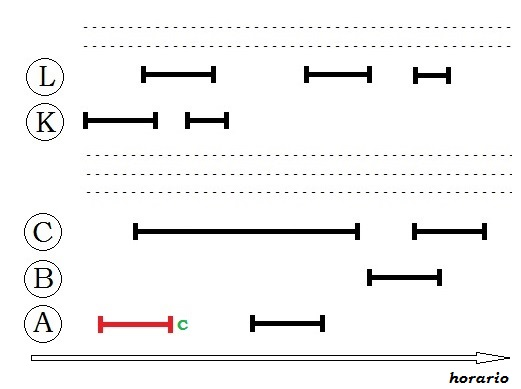
\includegraphics[scale=0.60]{imagenes/demo3.jpg}
	\end{center}
\end{figure}\\
Ahora, posicionados en C, realizar la búsqueda binaria de vuelos de salida de C hará que no consultemos vuelos que obviamente no podemos tomar (como el primer vuelo largo de C), haciendo que nos concentremos en el siguiente.
\begin{figure}[h]
	\begin{center}
	   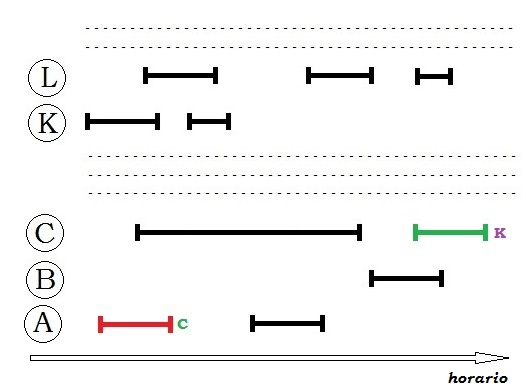
\includegraphics[scale=0.50]{imagenes/demo5.jpg}
	\end{center}
\end{figure}\\
Luego, dicho vuelos llevará nuestra atención a la ciudad K\\ Como nuestra busqueda binaria tiene 2 verificadores previos (explicado al inicio de la sección de complejidad), para el caso de ejemplo la búsqueda de vuelo se resuelve en O(1), viendo que no hay vuelos disponibles a la hora en la que llegamos a K.\\
Eso hace que volvamos a C para buscar otro vuelo, y a falta de otro para verificar, concluímos que a la hora de llegada a C (horario de llegada del primer vuelo de A) no es posible llegar hasta B (nuestro objetivo), por lo que guardamos en caché y procedemos a buscar otro vuelo en A.
\begin{figure}[h]
	\begin{center}
	   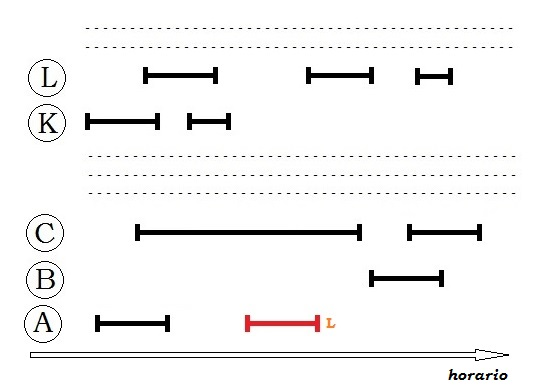
\includegraphics[scale=0.50]{imagenes/demo6.jpg}
	\end{center}
\end{figure}\\
Nuevamente, recursivamente llamamos a la ciudad J (ciudad disponible), y con búsqueda binaria, tomamos el primer vuelo posible.
\begin{figure}[h]
	\begin{center}
	   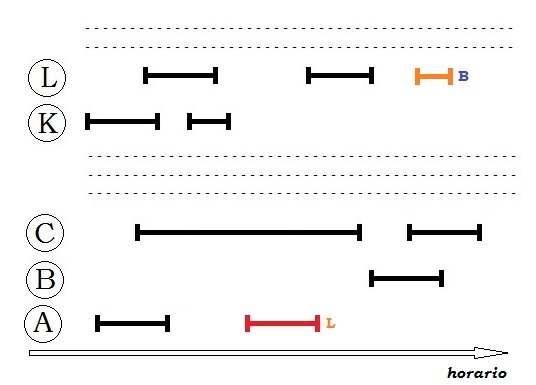
\includegraphics[scale=0.50]{imagenes/demo8.jpg}
	\end{center}
\end{figure}\\
Al tener ese vuelo como destino a B, guardamos en caché['L'] que desde L es posible llegar a B al horario de llegada del segundo vuelo de A, para no recalacularlo, y volvemos a A buscando otro vuelo que talvés nos termine llevando a B más temprano; como no lo hay, finaliza.

Si para el segundo vuelo de A, también hubieramos llegado a C, debido a que en cada ciudad se revisan los vuelos solo desde los que se pueden tomar hasta el ultimo sin revisar, \textbf{no hubieramos re-calculado el vuelo que se estaría tentado de calcular}, ya que la matriz caché indica que hay un calculo ya hecho a esa hora y simplemente basta con leerlo.\\
Ahora, si el segundo vuelo de A hubiera llegado lo suficientemente temprano como para tomar otro posible potencial vuelo de C,     caché['C'] \textit{pisaría} su valor para indicar la nueva franja horaria desde la que ya se conocen cálculos. 

Dicho eso, el peor de los casos, debido a sucesivos llamados recursivos podría acotarse superiormente por n búsquedas binarias, es decir, el peor caso del segundo submódulo tendría una cota superior \textbf{\textit{ O(n log n)}}.

\textit{\textbf{Notar que:}} la complejidad recién señalada, sugiere que se realizarían n búsquedas binarias (una por cada vuelo) de costo \textit{O(log n)} cada una, lo cual solamente pasaría si en todas las ciudades donde un vuelo llegara hubiera n vuelos de salida, lo cual es \textit{absurdo} ya que hay n vuelos en total y no hay vuelos que salgan y lleguen a la misma ciudad.\\
El único caso en el que se realizarían n búsquedas binarias sería que cada ciudad tenga solamente un vuelo de salida, pero, de darse ese caso, las mencionadas n búsquedas binarias se resolverían en O(1) cada una ya que el vector de vuelos de salida de cada ciudad tendría longitud = 1, resultando una complejidad \textit{O(n * 1) = O(n)}.\\
Por lo que \textit{\textbf{O(n log n)}} es una buena cota superior para el submódulo 2 de todo el programa.\\

\textit{\textbf{\underline{Análisis de mejor caso del submódulo 2}}}\\
Como el algoritmo se resuelve con la forma top-down, al comenzar mirando los vuelos de salida de A, esto hace que el mejor caso de este submódulo sea que \textbf{no salgan vuelos desde A}, teniendo una cota superior (de mejor caso) \textit{\textbf{O(1)}}.\\ \\

\noindent \underline{\textbf{\textit{Habiendo demostrado la complejidad de los 2 submódulos, la complejidad TOTAL del algoritmo es:}}} \\ \\
\textit{Complejidad submódulo 1 + Complejidad submódulo 2} = \\ \\
\textit{O(n log n) + O(n log n)} = \\ 

\noindent \textbf{\textit{O(n log n)}}\\ \\
\_\_\_\_\_\_\_\_\_\_\_\_\_\_\_\_\_\_\_\_\_\_\_\_\_\_\_\_\_\_\_\_\_\_\_\_\_\_\_\_\_\_\_\_\_\_\_\_\_\_\_\_\_\_\_\_\_\_\_\_\_\_\_\_\_\_\_\_\_\_\_\_\_\_\_\_\_\_\_\_\_\_\_\_\_\_\_\_\_\_\_\_\_\_\_\_\_\_\_\_\_\_\_\_\_\_\_\_\_\_\_\_\_\_\_\_\_\_\_\_\_\_\_\_\_\_\_\_\_\_\_\_\_\_\_\_\_\_\_\_\_
\\

\noindent \textit{\underline{\textbf{Demostración propiedad:}} Complejidad Ordenar subarreglos = Complejidad Ordenar arreglo entero}\\

\noindent \textbf{Sean} \textit{X,Y} y \textit{Z} arreglos tal que X.size() + Y.size() + Z.size() = n.\\
\textbf{Sea} \textit{tamI} el tamaño de un arreglo I. (Ej: tamX = X.size())\\
\textbf{Sea} sort() un algoritmo que ordena colecciónes tal que la complejidad de ordenamiento es O(coleccion.size() * log coleccion.size()) cuando el acceso a una posición de la colección se realiza en O(1).\\

\noindent Entonces, ordenar X, Y y Z con \textit{sort()} toma:

\indent \textit{\textbf{O(tamX * log tamX)}} + \textit{\textbf{O(tamY * log tamY)}} + \textit{\textbf{O(tamZ * log tamZ)}}\\

\noindent Como tamX + tamY + tamZ = n, entonces:

\indent (tamX * log tamX) \textless = (n * log n)\\
\indent (tamY * log tamY) \textless = (n * log n)\\
\indent (tamZ * log tamZ) \textless = (n * log n)\\

\noindent Luego, podemos acotar la complejidad mencionada anteriormente:

\indent \textit{\textbf{O(n log n)}} + \textit{\textbf{O(n log n)}} + \textit{\textbf{O(n log n)}} = \textit{3*\textbf{O(n log n) = O(n log n)}}\\

\noindent Quedando así demostrado que ordenar k subarreglos tal que la suma de sus longitudes es n, tiene una complejidad \textbf{O(n log n)}.

\newpage
\subsection{Experimentación}

\noindent Para el proceso de experimentación del problema se plantearon distintas pruebas para corroborar que el algoritmo propuesto funcionara correctamente, y que la cota de complejidad encontrada y justificada en la sección anterior, se cumpliera en la práctica.\\

\noindent Dado que el CPU de la computadora utilizada para tomar los tiempos no está atendiendo únicamente a nuestro proceso, realizar una sola vez cada prueba podría darnos valores que no son cercanos a los reales. Por lo tanto, para minimizar este margen de error, a cada prueba se la hizo ejecutar un total de 100 veces, y se tomó el mejor valor, es decir, el menor tiempo de ejecución obtenido. Notar que, tomar el mejor valor no es una mala decisión, ya que cuanto más chico sea el valor, más cerca estamos del valor real de tiempo que toma el algoritmo para una instancia dada.\\

\noindent En cada prueba, se tomaron métricas para la posterior evaluación del algoritmo en la práctica. Vale aclarar que la medición no contempla tiempos de salida de datos, sino que contempla:\\

\noindent \begin{enumerate}
\item La preparación de los datos de entrada para su procesamiento
\item El algoritmo que determina el mejor itinerario posible.\\
\end{enumerate}

\noindent Para el testeo, se diseñó un generador de instancias aleatorias que toma dos parámetros:\\


\noindent \begin{enumerate}
\item \textbf{Cantidad de ciudades:} determina cuántas ciudades se tomarán aleatoriamente que puedan ser origen o destino de los vuelos, seteando por lo menos un vuelo a cada una o desde cada una para que sean ciudades con sentido.

\item \textbf{La cantidad de vuelos presentes en la instancia}.\\
\end{enumerate}

\noindent Con este programa pudimos evaluar cuánto tiempo de ejecución toma nuestro algoritmo para distintas instancias aleatorias del problema.\\

\noindent Para todos los casos, se eligió una precisión de hasta 0,0001 ms (milisegundos). De ser menor, la tomamos como 0.\\

\noindent También desarrollamos un programa similar al explicado anteriormente, pero que arroja únicamente instancias de mejor caso.\\

\noindent Finalmente, el proceso de testing es:\\


\noindent \begin{enumerate}
\item Generación de instancia aleatoria, según parámetros prefijados.
\item Ejecución de dicha instancia 100 veces, tomando el mejor tiempo obtenido.
\item Repetición de los items 1 y 2 otras 99 veces y obtención del tiempo promedio.
\end{enumerate}

\noindent Con esta metodología de experimentación, realizamos pruebas en dos tipos de escenarios:\\
\noindent \begin{itemize}
\item Escenarios de casos aleatorios
\item Escenarios de mejor caso\\
\end{itemize}

\noindent A continuación, describiremos las particularidades de cada escenario.


\subsubsection{Escenarios de casos aleatorios}

\noindent En estos escenarios, decidimos evaluar casos aleatorios, generados por el generador de instancias aleatorias descripto anteriormente.\\

\noindent La idea fue tomar muestras del algoritmo haciendo variar la cantidad de vuelos, generando instancias que den origen y destino aleatorio a los mismos.\\

\noindent Para poder diferenciar bien los casos y poder analizar mejor, decidimos que cada escenario de las pruebas de caso aleatorio tenga una cantidad de ciudades constante. Esta capacidad de ciudades fue prefijada de manera que, si establecemos una cantidad m de ciudades, haya por lo menos un vuelo que salga o llegue a cada una, para que en la instancia haya por lo menos m ciudades activas.\\

\noindent A continuación, los gráficos resultantes de la experimentación en estos escenarios. Para los mismos, variamos la cantidad de vuelos aumentándolos de a 100 y elegimos probar con 20, 40 y 80 ciudades.\\

\noindent Para cada una de las pruebas, mostraremos la tabla con los valores obtenidos, los análisis de tiempos de ejecución y un análisis gráfico para estimar la complejidad del algoritmo.\\

\noindent \textit{Aclaración: Por simplicidad, nos referiremos de ahora en más con \textbf{n} a la \textbf{Cantidad de vuelos}. \\\\
}
	\begin{figure}[h]
		\begin{center}
		   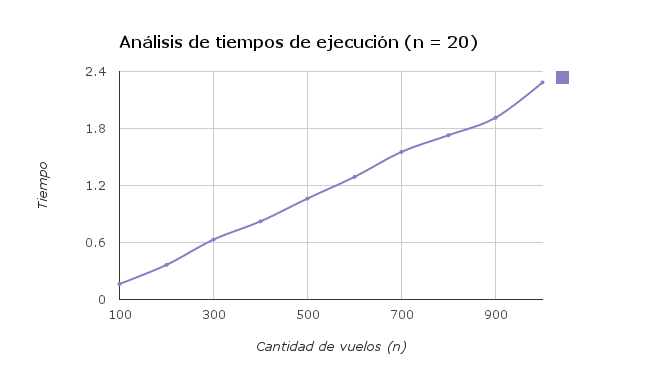
\includegraphics[scale=0.75]{graficos/tiempo_ejecucion20.png}
		\end{center}
	\end{figure}

\newpage
	\begin{figure}[h]
		\begin{center}
		   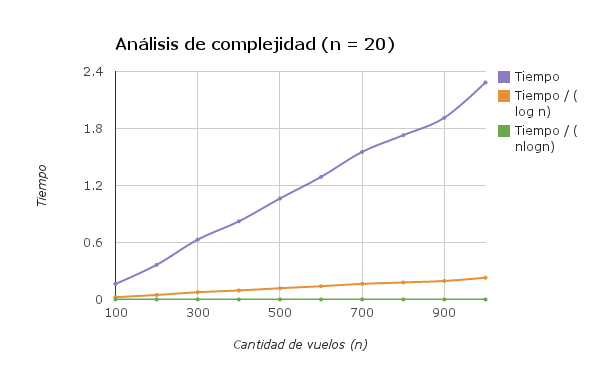
\includegraphics[scale=0.75]{graficos/complejidad_20.png}
		\end{center}
	\end{figure}



	\begin{figure}[h]
		\begin{center}
		    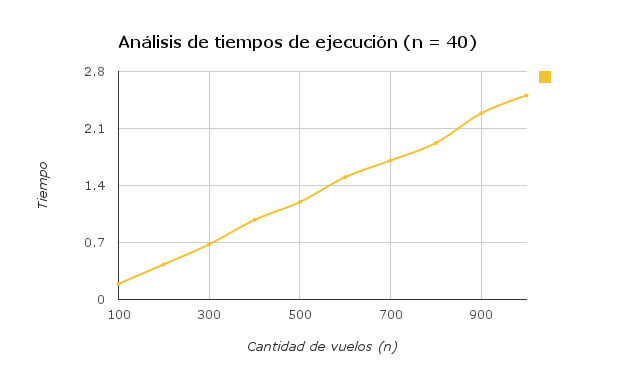
\includegraphics[scale=0.75]{graficos/tiempo_ejecucion40.png}
		\end{center}
	\end{figure}

\newpage


	\begin{figure}[h]
		\begin{center}
		   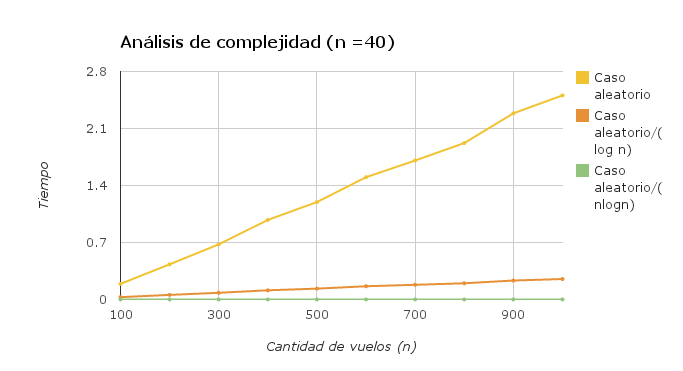
\includegraphics[scale=0.75]{graficos/complejidad_40.png}
		\end{center}
	\end{figure}


	\begin{figure}[h]
		\begin{center}
		   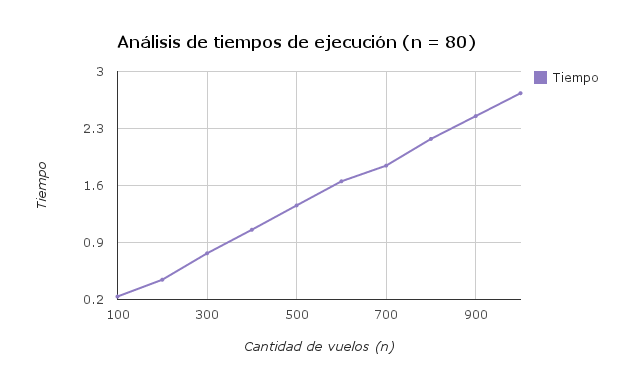
\includegraphics[scale=0.75]{graficos/tiempos_80.png}

		\end{center}
	\end{figure}

\newpage

	\begin{figure}[h]
		\begin{center}
		   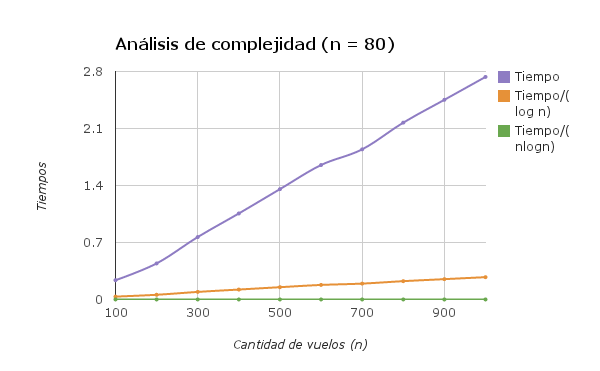
\includegraphics[scale=0.75]{graficos/complejidad_80.png}
		\end{center}
	\end{figure}

\subsubsection{Escenario de mejor caso}

\noindent En este escenario, realizamos una experimentación análoga a la detallada anteriormente: generamos instancias de mejor caso, haciendo variar la cantidad de vuelos aumentándolos de a 100, y dejando fija la cantidad de ciudades, de la misma forma en que se explicó en el escenario anterior. Sin embargo, en este caso, únicamente realizamos la experimentación considerando 40 ciudades. \\\\
	\begin{figure}[h]
		\begin{center}
		   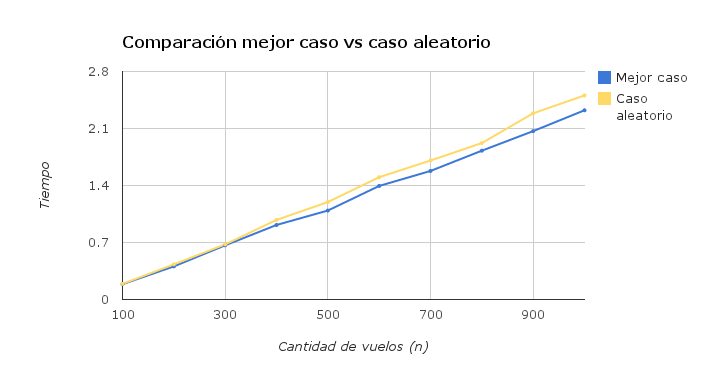
\includegraphics[scale=0.75]{graficos/comparacion_mejorcasoCasoAleatorio.png}
		\end{center}
	\end{figure}

\newpage
	\begin{figure}[h]
		\begin{center}
		   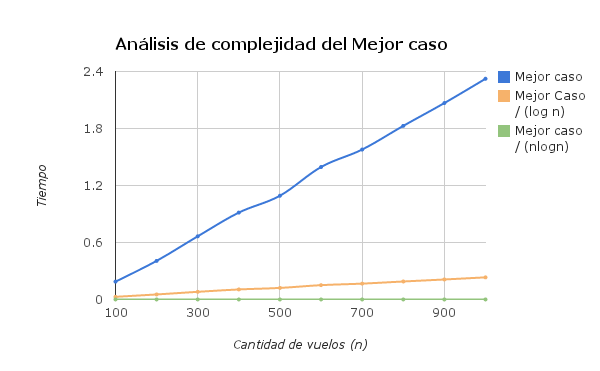
\includegraphics[scale=0.75]{graficos/complejidad_mejorCaso.png}
		\end{center}
	\end{figure}


\subsubsection{Conclusiones}
\textit{Aclaración: En esta sección continuamos refiriéndonos con \textbf{n} a la \textbf{Cantidad de vuelos}.}

\noindent Corroboramos lo analizado analíticamente, verificando en lo empírico que la complejidad del algoritmo propuesto es O(n log n).\\
\noindent En los gráficos de complejidad presentados en los distintos escenarios vemos claramente que al dividir punto f(n) de la función por log n nos queda una función lineal, y al hacerlo por n log n una constante. Esto solo podria pasar si efectivamente la curva que obtenemos al graficar los tiempos medidos está acotada por O(n log n).\\
\noindent Comprobamos además que a partir de la comparación de los gráficos obtenidos con instancias de 20, 40 y 80 ciudades, que la medición de tiempos, arroja para cualquiera de los tres escenarios curvas acotadas por O(n log n), por lo que corroboramos lo que analizamos desde lo analítico: la complejidad temporal del algoritmo no reside en la cantidad de ciudades que se usen para realizar los vuelos, si no en la cantidad de los mismos. Esto se debe a lo ya enunciado en el apartado de complejidad, donde expusimos que la cantidad de ciudades es del orden de n, ya que a lo sumo hay 2.n + 2 ciudades.\\
\noindent Por otro lado, en tanto al caso propuesto como mejor, observamos que arroja para cada n una medición de tiempo mejor que para una instancia de mismo n, pero de caso aleatorio. Sin embargo, este mejor caso solo impacta el cálculo de mejor camino, y no así la preparación de los datos, por ende esta curva obtenida a partir de la experimentación con instancias de mejor caso es también acotada por O(n log n), solo que con mejores tiempos debido a constantes de multiplicación menores.\\
\noindent De esta forma, corroboramos lo analizado analíticamente.\\

\end{document}
% Fin Ejercicio 1

\newpage
% Comienzo Ejercicio 1
\documentclass[10pt,a4paper]{article}
\usepackage[utf8]{inputenc} % para poder usar tildes en archivos UTF-8
\usepackage[spanish]{babel} % para que comandos como \today den el resultado en castellano
\usepackage{fullpage} %small margins
\usepackage[parfill]{parskip} %genera saltos entre parrafos
\usepackage{color}
\definecolor{gray}{gray}{0.35}
\usepackage{listings}
\usepackage{enumitem}
\usepackage{amsmath} %big brackets
\usepackage{mathtools}
\lstset{
    numbers=left,
    breaklines=true,
    tabsize=2,
    basicstyle=\ttfamily\color{gray},
}
\setlength{\parindent}{8pt}
\usepackage{mathtools}
\usepackage[margin=50pt]{geometry}
\usepackage{amsfonts}
\usepackage{flafter}
\usepackage{multicol}

\begin{document}

\section{Algoritmo exacto}
\subsection{Desarrollo}
El problema que se nos presenta es el de la k-PMP. El mismo trata sobre, dado un grafo G=(V,E) con pesos en las aristas, encontrar una particion de los nodos en k (o menos) conjuntos, tal que sea la partición de menor peso.
Lo que hace al peso de una partición, es la suma de los pesos de las aristas intrapartición (sin importar aquellas que no lo son). Una arista se dice \textit{intrapartición} cuando los 2 nodos sobre los que incide pertenecen al mismo conjunto de partición.\\

Dicho esto, para la realización del algoritmo exacto, optamos por revisar todas las particiones posibles de los n nodos, y quedarnos con la mejor (la de menor peso) de las que tengan k o menos conjuntos.
Se elaboraron podas y estrategias previas al analisis de todas las posibles particiones para mejorar los tiempos de ejecución, y mejorar la complejidad espacial.\\

\textbf{\underline{\textit{Nota:}} A lo largo de todo el desarrollo del algoritmo exacto, cuando se hace referencia a\\ \textbf{\textit{"particionesDeN"}} es una forma abreviada de hablar de las particiones del conjunto \{1,2,3,...,n\}} \\

El algoritmo \textit{\textbf{sin podas ni estrategias}} para generar las particiones de un conjunto de n nodos es el siguiente:

Si Miramos las particiones de un conjunto de 1, 2, y 3 elementos:

\begin{figure}[h]
	\begin{center}
	   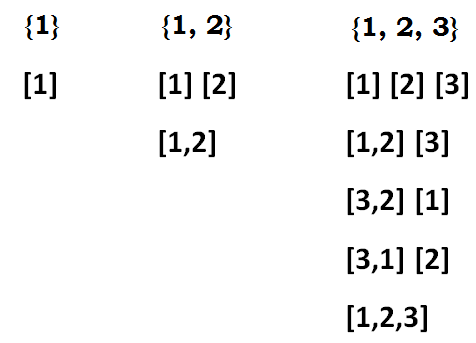
\includegraphics[scale=0.7]{ParticionesNegro.png}
	\end{center}
\end{figure}
Y si notamos la siguiente similitud entre la transición de uno a otro (ejemplo, transición de particionesDe2 a \\particionesDe3):\\
\begin{figure}[h]
	\begin{center}
	   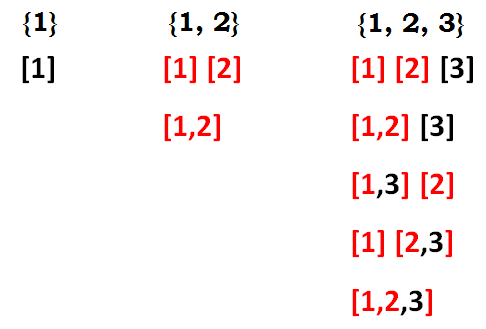
\includegraphics[scale=0.7]{ParticionesNegroRojo.png}
	\end{center}
\end{figure}\\
Veremos que las particionesDe3 son las particionesDe2 solo que agregando el 3  primero en un subconjunto aparte, y luego dentro de los subconjuntos de 2. Entonces:

\newpage
Para generar las particiones un conjunto de 3 elementos, a partir de las particiones de un conjunto de 2 elementos, hace 2 pasos:\\
\begin{enumerate}
\item Toma todas las de 2 elementos y le agrega un nuevo conjunto que solo contiene al 3 (en el gráfico, las 2 primeras particiones), ese nuevo grupo de particiones ya formará parte de las particiones finales de 3 elementos.\\
Esta cantidad de particiones añadidas cumple que \#particionesAñadidas = \#particionesTotalesDeN-1
\begin{figure}[h]
	\begin{center}
	   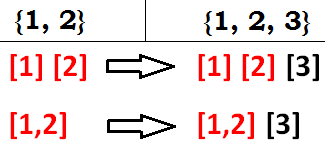
\includegraphics[scale=0.6]{explicacionPaso1.png}
	\end{center}
\end{figure}\\


\item Luego, vuelve a mirar las particiones de 1..2, y por cada una (llamemosle X) realizará lo siguiente:\\
\indent Añadirá una partición por cada subconjunto de X, y en cada una de ellas, agregará el valor de n (3 en este caso) a un subconjunto distinto para luego formar parte de las particiones finales buscadas.\\
\begin{figure}[h]
	\begin{center}
	   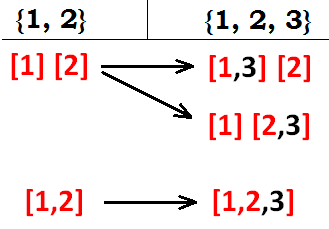
\includegraphics[scale=0.6]{explicacionPaso2.png}
	\end{center}
\end{figure}\\

\indent \textbf{\underline{Ej:}} Toma la partición \textbf{[1] [2]}:\\
\indent -Aplica el \textbf{3} al subconjunto \textbf{[1]}, quedando: \textbf{[1,3] [2]} que ya formará parte de las particiones finales.\\
\indent -Agrega a las particiones finales.\\
\indent -Revierte el 3 aplicado.\\
\indent -Luego aplica el \textbf{3} al subconjunto \textbf{[2]} de la misma partición, resultando en el conjunto: \textbf{[1] [2,3]}\\
\indent -Agrega a las particiones finales.

Y así se construyó la tercer y cuarta partición; repitiendo el procedimiento para la partición \textbf{[1,2]} se obtendrá la última partición de las 5.\\
\end{enumerate}
Esa es la \textbf{base} del algoritmo exacto utilizado para generar las particiones de un conjunto de números de tamaño n. Se deja guardada en el código la partición base, que es la única partición de un conjunto de 1 elemento, y para las demás se realiza el procedimiento mencionado n-1 veces, generando así las particiones de un conjunto de n elementos a partir de las de un conjunto de n-1.\\
Tiene una gran \textit{'pinta'} recursiva, pero decidimos hacerlo iterativo.\\

A continuación, el pseudocódigo del algoritmo (nuevamente, sin las podas):\\

\textbf{subConjunto} es un vector\textless Enteros\textgreater \\
\indent \textbf{Particion} es un vector\textless subConjunto\textgreater\\
\indent \textbf{PARTICIONES} es un vector\textless Particion\textgreater

\newpage
\underline{Recibe:}\\
-Un conjunto de particiones que esta vacío para que lo llene.\\
-El n
\begin{lstlisting}
getPartitionsOfN(n, PARTICIONES)

		PARTICIONES := {{1}}
	
		for i = 2 to n inclusive do
			lengthAnterior := PARTICIONES.length

			for j = 0 to lengthAnterior inclusive do
				jPartition := copyOf(PARTICIONES[j])

				PARTICIONES[j] U {i}			
					
				for p = 0 to jPartition.length hacer
					jPartition[p].push_back(i).
					PARTICIONES U {jPartition}.
					jPartition[p].pop_back();
				Fin Para
			
			end for
	
		end for

		devolver PARTICIONES;

end of getPartitionsOfN
\end{lstlisting}
---------------------------------------------------------------------------------------------------------------------------------------------------

\underline{\textbf{Las podas y estrategias:}}

\begin{enumerate}
\item \textbf{Poda de cantidad de conjuntos.}\\
Dado un n, la cantidad máxima de conjuntos que puede tener una particion de n es n. Pero las particiones de n tales que tienen mas de k conjuntos no nos interesan, ya que estamos en el problema de la k-PMP donde nos interesan las particiones que tengan a lo sumo k conjuntos.\\
Ejemplo utilizando las imágenes usadas para la explicación del algoritmo; en ese caso, n = 3. Si nuestro k (por ejemplo) es 2, ¿tendría sentido agregar la primer particion al conjunto de particiones final ([1][2][3])? No lo tendría puesto que por definición de una k-PMP no puede ser una solución del problema, y estaríamos generando particiones que luego analizariamos cuando ya sabemos de antemano que no son posibles.\\

\item \textbf{Poda de mejor peso encontrado hasta el momento.}\\
Esta poda se basa en que el peso de cualquier partición de n que tenga k o menos conjuntos es\textgreater = al peso de la solución óptima.
Dicho esto, si supieramos que alguna particion de n (y tamaño\textless = k) tiene peso X, entonces cuando estamos construyendo las particiones, si notamos que la particion que estamos construyendo ya sobrepasó ese límite (a pesar de que aún no tenga los n elementos), entonces no tiene sentido seguir construyendola ya que el peso intraparticion de los elementos ya aplicados lo superó y por lo tanto no es óptima. Si esto ocurre, se elimina esa partición de el conjunto de particiones credas hasta el momento.
Este valor X lo conseguimos mediante una \textit{cota inicial} que realizamos previo a la formación de las particiones de n, que será explicado en breve.\\

\item \textbf{Poda de actualización de mejor peso encontrado.}\\
En la poda recién explicada, se detallaba que dado un peso X calculado anteriormente, las particiones que se estén construyendo y alcanzaran dicho límite serían removidas. Pero ¿por qué no ir actualizando este límite si vamos encontrando particiones tales que ya tienen todos los nodos cargados y mejor peso que X?\\
Eso es lo que hace esta poda, si dada una partición U de n, tal que peso(U)\textless peso\_optimo\_parcial, entonces peso\_optimo\_parcial = peso(U). Esto permitirá que más particiones sean recortadas a futuro.\\
\textit{Aclaración:} Como se explicó, esta cota tiene utilidad recién cuando se encuentra una particion n. En nuestro algoritmo, no nos sirve mientras estamos construyendo las particiones de n-1, n-2,...,3,2 ya que necesitamos todos los nodos cargados para poder asegurar que encontramos un peso tal que peso\textless peso\_optimo\_parcial. Por ende somos conscientes que hasta la última iteración del for principal (pseudocódigo) no nos sirve, pero debido a que el peso de una partición actual en construcción ya lo calculamos para la poda anterior (poda número 2) realizar el checkeo y la asignación es O(1), así que no perdíamos nada por aplicarla.\\

\item \textbf{Estrategia previa para acotar el peso de la solución óptima.}\\
En esta estrategia, para obtener una cota superior de lo que puede llegar a pesar la solución óptima, decidimos ejecutar el algoritmo goloso antes del exacto (ejercicio 3 de este Trabajo Práctico) para que nos devuelva una configuración posible de los nodos (potencialmente óptima) y tomar su peso para usarlo como cota en la construcción de las particiones.\\
Si la cota devolviese la peor solución habría sido como si no hubiera existido, porque no hubiera acotado al problema.\\
\end{enumerate}

Dicho esto, a continuación el pseudocódigo \textit{con podas} de la parte del algoritmo que se encarga de la construcción de las particiones:\\

\begin{lstlisting}
getPartitionsOfN(pesos, n, k, PARTICIONES)

		PARTICIONES := {{1}}
	
		para i desde 2 hasta n inclusive hacer
			lengthAnterior := particiones.length

			para j desde 0 hasta lengthAnterior inclusive hacer		
				copy := copyOf(j-esima particion de PARTICIONES)

				Si la j-esima particion aun no tiene tamano igual a k
					agregar conjunto {i} a la j-esima particion			
				Sino
					Borrar la j-esima particion de PARTICIONES;
					j--;
					lengthAnterior--;
				Fin si
			
				Para p desde 0 hasta copy.length - 1 inclusive hacer
					copy[p].push_back(i);
					peso := peso(copy);
					
					Si peso < optimo_peso_parcial		
						Agregar copy a PARTICIONES
						Si i == n
							optimo_peso_parcial <- peso;					
						Fin Si
					Fin Si
					
					copy[p].pop_back();
					
				Fin Para
			
			Fin para
	
		Fin para

		return;

end of getPartitionsOfN
\end{lstlisting}
---------------------------------------------------------------------------------------------------------------------------------------------------
\newpage
\subsection{Análisis de la complejidad temporal}
Para la ejecución de la implementación del algoritmo (en C++), veremos el algoritmo en su peor caso, que es \textbf{sin ninguna cota aplicada}.\\
También, para los casos donde se realize el método push\_back() de la clase vector, si bien su costo es\\ \textbf{O(1) amortizado}, para simplificar el analisis de complejidad, se tomará como O(1).\\

Tenemos 3 ciclos a mirar.\\

\noindent \underline{El \textbf{primer ciclo for}}:\\
Itera un total de n-1 veces. Como es el for "padre", la complejidad temporal final será:

\textit{O(costo iteración 1) + O(costo iteración 2) + ... + O(costo iteración n-1)}. $\forall$\textit{n\textgreater =2}\\

\noindent Veamos el costo de cada iteración:

Se ejecuta solamente una asignación y \textbf{el segundo for}, por lo que la complejidad de cada iteración será igual a la complejidad de dicho segundo for en la misma iteración (la asignación es en O(1)). Veamoslá:\\

\noindent \underline{El \textbf{segundo ciclo for}}:\\
El for cicla tantas veces como la variable \textbf{lengthAnterior} indique.\\
Como dicha variable toma el tamaño de PARTICIONES, que al principio de cada iteración i del primer for contiene todas las particiones del conjunto \textit{\{1,2..i-1\}}, entonces la complejidad de dicho for será:

\textit{ O(\#particionesDeI-1 * costo de cada iteración del segundo for)}.

\noindent Veamos ahora el costo de cada iteración del segundo for.

\begin{enumerate}
\item Realizar el backup de una partición tiene costo \textit{O(n)} puesto que a lo sumo tiene a todos los nodos, es decir, n nodos.
\item Acceder a la j-esima posición de PARTICIONES y modificarlo agregandole un subConjunto tiene costo O(1).
\item Por último tenemos el costo del último for (tercer for), que itera los subConjuntos de la particion backupeada.
\end{enumerate}
Por lo que la complejidad temporal del segundo for en una iteración es:\\
\textit{O(n + costo del tercer for)}\\

\noindent \underline{El \textbf{tercer ciclo for}}:\\
Dada la j-esima partición backupeada en el segundo for, itera todos los subConjuntos. En el peor caso una partición puede tener n subConjuntos (1 nodo en cada uno), por lo que el costo es:\\
\textit{O(n * costo de cada iteración)}.

\noindent Donde el costo de cada iteración es:
\begin{enumerate}
\item Acceder a un conjunto y agregar un elemento: \textit{O(1)}.
\item Copiar la particion backupeada a PARTICIONES: \textit{O(n)}.
\item Acceder al último conjunto modificado y eliminar el elemento recién agregado: \textit{O(1)}.
\end{enumerate}
Costo final de cada iteración: \textit{O(n)}.\\

\noindent Por ende, el costo final \textbf{(de peor caso)} del tercer for es:

\textit{\textbf{O(n * n) = O($n^2$)}}\\ \\

Ahora, reemplazando la cota de complejidad conseguida del tercer for en el costo de \textbf{cada iteración del segundo for} nos queda:

\textbf{\textit{O(n + costo del tercer for) = O(n + $n^2$) = O($n^2$)}}

\noindent Volviendo a la complejidad del segundo for en una iteración i del primer for, teníamos:

\textit{O(\#particionesDeI-1 * costo de c/iteración del segundo for)}. = \textbf{\textit{O(\#particionesDeI-1 * $n^2$)}}

\newpage
Volviendo a la complejidad del primer for, teníamos que el costo total del algoritmo era:

\textit{O(costo iteración 1) + O(costo iteración 2) + ... + O(costo iteración n-1)}. $\forall$\textit{n\textgreater =2}\\
Donde \textit{costo iteración i} es el costo del segundo for en la iteración i del primer for.\\

Reemplazando lo conseguido del análisis del segundo for, el costo total del algoritmo es:

\textbf{\textit{O(\#particionesDe1 * $n^2$)) + O(\#particionesDe2 * $n^2$) + ... + O(\#particionesDeN-1 * $n^2$)}}.\\



\underline{Analizando la cantidad de particiones posibles distintas de un conjunto de N elementos.}\\
Los \textbf{\textit{Números de Bell}} (http://en.wikipedia.org/wiki/Bell\_number) son los números que indican la cantidad de particiones distintas posibles de un conjunto dado. Los mismos fueron presentados por \textit{Eric Temple Bell} y se definen bajo la siguiente fórmula \textbf{recursiva}:\\

INSERTE LATEX AQUI DE LA FORMULA DE BELL.\\

Se conocen distintas cotas superiores de estos números (http://en.wikipedia.org/wiki/Bell\_number\#Growth\_rate), y la que vamos a usar es la establecida por \textit{Berend. y Tassa. (Improved Bounds on Bell Numbers and on Moments of Sums of Random Variables)}, la cual acota superiormente al termino Bn de los números de Bell por la siguiente relacion:\\

INSERTE LATEX AQUI DE LA COTA.\\ \\


\noindent Luego, como la cantidad de particiones de un conjunto es estrictamente creciente en el tamaño del mismo, volviendo a donde habíamos quedado con respecto a la complejidad total del algoritmo:

\noindent \textit{O(\#particionesDe1 * $n^2$)) + O(\#particionesDe2 * $n^2$) + ... + O(\#particionesDeN-1 * $n^2$)} $\in$

\noindent \textit{O((n-1) * (\#particionesDeN-1 * $n^2$))} $\in$ 

\noindent \textit{O($n^3$ * \#particionesDeN-1)} $\in$ (Usando la cota mencionada)

\noindent \textit{O($n^3$ * $((n-1)/ln(n-1+1))^n$)}.\\

Finalmente, removiendo constantes:

\textbf{\textit{O($n^3$ * $(n/ln(n))^n$)}} que es una cota de la complejidad temporal final del algoritmo\\ \\ \\

\underline{\textbf{Análisis con las podas aplicadas}}

Las podas aplicadas al algoritmo en sí (dejando de lado la ejecución previa del algoritmo goloso) son las 3 primeras mencionadas anteriormente.

Para la \textbf{primer poda}, se agregó un if que en cada iteración del segundo for consulta por el tamaño actual de la partición para evitar revisar particiones de más de k conjuntos.\\
Dado que el método \textit{.size()} de vector es en \textit{O(1)}, la guarda del if se ejecuta en tiempo constante.\\
Si se ingresa por el if la ejecución continúa su flujo normal, de lo contrario, se hacen 2 operaciones básicas y un borrado, el cual en peor caso tiene costo \textit{O(n)}, por lo que no modifica la complejidad ya que previo a eso se había invertido O(n) en copiar la instancia, y porque el mayor costo lo tiene el tercer for con \textit{O($n^2$)}.\\
Eliminar dicha instancia evita que se siga ramificando apartir de ella un subárbol de desiciones que crece exponencialmente y que no tiene sentido revisar.\\
También, evitando generar esas particiones no solo ganamos temporalmente, sino también (en la práctica) en la espacialmente.

Para la \textbf{segunda poda}, se hace la medición del peso de la partición durante el tercer for antes de agregarla al conjunto de particiones final. Esta validación no se hace cuando se agrega un conjunto nuevo aparte (antes del tercer for) ya que agregar un conjunto con un solo elemento no modifica el peso de las aristas intrapartición.\\
Calcular el peso de la partición tiene costo \textit{O($n^2$)}, por lo cual, teóricamente estamos perdiendo complejidad, ya que cada iteración del tercer for ya no cuesta \textit{O(n)}, sino \textit{O($n^2$ + n) = O($n^2$)}, pero en la práctica favoreció de una manera muy positiva cuando trabaja en conjunción con la cota superior dada por el algoritmo goloso.

Finalmente para la \textbf{tercer poda}, se hace la actualización del peso\_optimo\_parcial. Esto se realiza mediante un if con una guarda que se ejecuta en \textit{O(1)}, al igual que el cuerpo del mismo.\\
Esto es así ya que el peso de la partición lo teníamos calculado y guardado cuando lo utilizamos en la segunda poda.\\

\noindent En conclusión, las podas no empeoraron la complejidad del algoritmo, a excepción de la poda numéro 2, que si bien, por el análisis teórico transforma \textit{O(n)} en \textit{O($n^2$)}, trabajando conjuntamente con el algoritmo goloso ejecutado previamente, es la poda que más eficiencia nos provió.\\
El caso en el que esta poda no tenga efecto positivo sobre el algoritmo y finalmente termine siendo una contra, sería el caso en el que el algoritmo goloso devuelva la peor partición posible de los nodos, lo cual tiene una ínfima posibilidad de ocurrir.\\

\noindent \textbf{\textit{Nota: }} En cuanto al algoritmo goloso no se hace un análisis del mismo puesto que eso ya fue hecho en el ejercicio 3 de este trabajo práctico.\\Además, este presenta una complejidad polinomial, la cual es despreciable en comparación con las escalas de complejidad que ronda el algoritmo exacto en sí.




  
\newpage
\subsection{Experimentación}
Para la experimentacion, se realizaron distintos escenarios de test. Cada escenario contiene valores que son producto de distintas tomas de datos del algoritmo en ejecución.

Como es sabido, la computadora en la que se realizaron las mediciones, no está atentiendo nuestro proceso únicamente. Es por eso, que realizar una única medición de cada instancia no nos asegura fidelidad.\\
\indent Para aminorizar esta falencia, se repitió cada instancia de cada caso de test de cada escenario, un total de 10 veces, y se tomó el mejor tiempo.\\
Notar que tomar el mejor tiempo (en lugar del promedio) no es una mala desición, ya que entre 2 mediciones de tiempos distintas, t1 y t2, si t1\textless t2, eso nos asegura que en t1 el procesador estuvo más focalizado en nuestro proceso, y por ende, es una medición más fiel del mismo.

Para realizar las mediciónes, se realizó un generador de instancias aleatorias, que dada una cantidad de nodos (n), una cantidad de aristas (m) y un entero (k), genera de forma aleatoria m aristas, tomando para cada una, 2 nodos de n, que no tengan ya una arista entre ellos.

También, para el escenario de un k dado, no se hicieron pruebas donde ocurra que k\textgreater =n, ya que la respuesta de estos casos es trivial, (que cada nodo podría ir en un conjunto distinto). Hacer las mediciones de un caso trivial no tiene mucho sentido, por lo que en todas las mediciones, siempre vale que k\textless n.

En todos los casos se midieron grafos de n nodos, que tengan una densidad de aristas del 25\%, 50\%, 75\% y 100\%.

Los valores de k elegidos fueron 3, 5, 8 y 13, que siguen la serie de \textit{Fibonacci} para una variación más uniforme.\\

\underline{\textbf{Los escenarios:}}
\textbf{\textit{ESCENARIO CON K = 3:}}
	\begin{figure}[h]
		\begin{center}
		   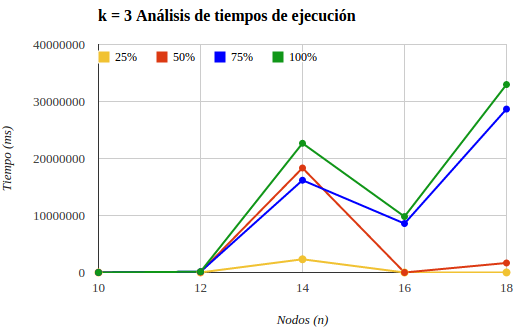
\includegraphics[scale=0.70]{graficos/k3.png}
		\end{center}
	\end{figure}\\
	\begin{figure}[h]
		\begin{center}
		   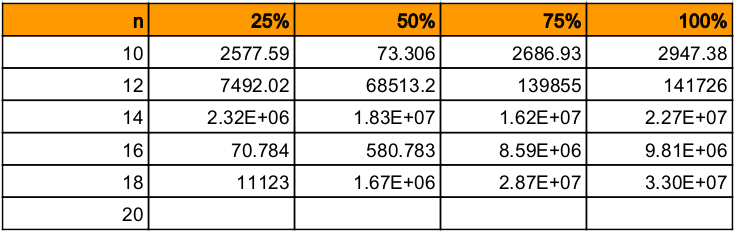
\includegraphics[scale=0.50]{graficos/tablak3.png}
		\end{center}
	\end{figure}\\

	
\newpage	
\textbf{\textit{ESCENARIO CON K = 5:}}
	\begin{figure}[h]
		\begin{center}
		   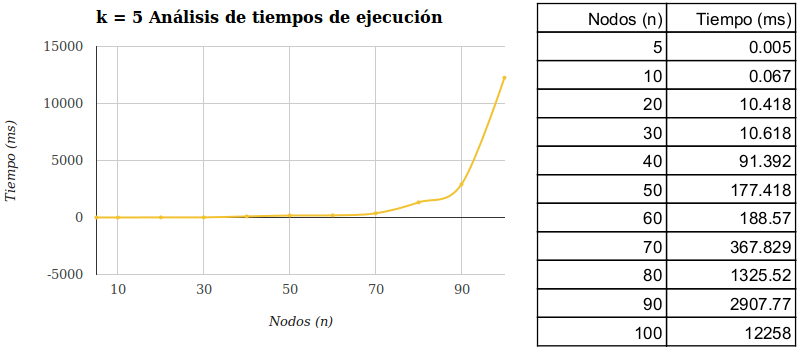
\includegraphics[scale=0.70]{graficos/k5.png}
		\end{center}
	\end{figure}\\
	\begin{figure}[h]
		\begin{center}
		   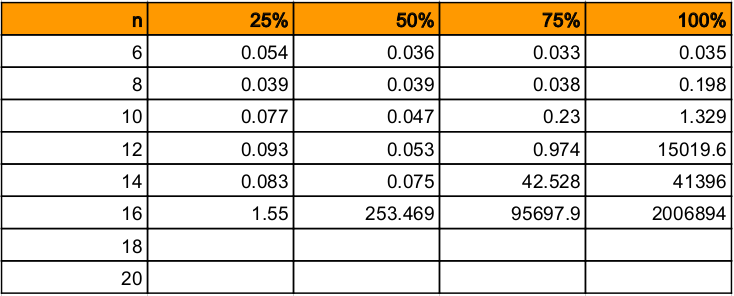
\includegraphics[scale=0.50]{graficos/tablak5.png}
		\end{center}
	\end{figure}\\
\newpage
\textbf{\textit{ESCENARIO CON K = 8:}}
	\begin{figure}[h]
		\begin{center}
		   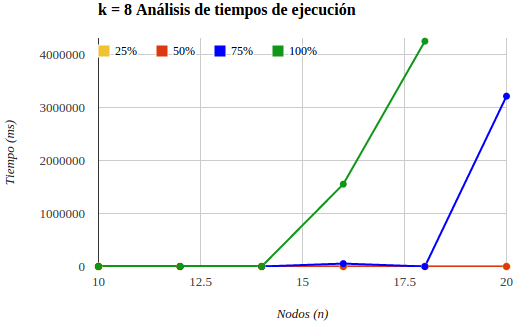
\includegraphics[scale=0.70]{graficos/k8.png}
		\end{center}
	\end{figure}\\
	\begin{figure}[h]
		\begin{center}
		   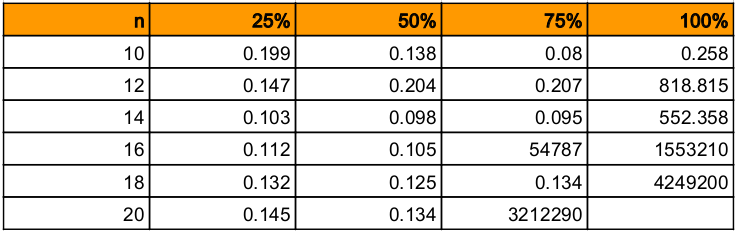
\includegraphics[scale=0.50]{graficos/tablak8.png}
		\end{center}
	\end{figure}\\
	
\newpage
\textbf{\textit{ESCENARIO CON K = 13:}}
	\begin{figure}[h]
		\begin{center}
		   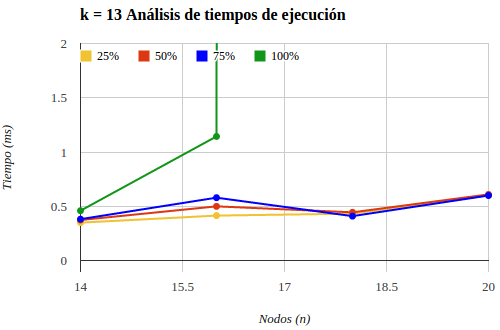
\includegraphics[scale=0.50]{graficos/k13ConZoom.png}
		\end{center}
	\end{figure}\\
\indent Si le alejamos un poco el zoom...
	\begin{figure}[h]
		\begin{center}
		   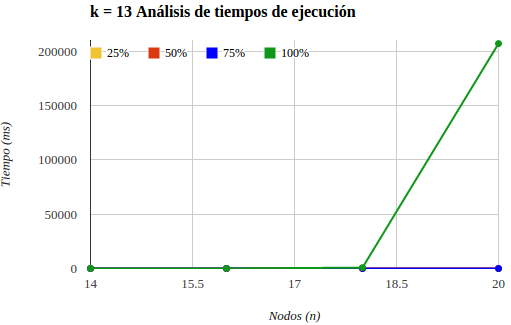
\includegraphics[scale=0.50]{graficos/k13SinZoom.png}
		\end{center}
	\end{figure}
	\begin{figure}[h]
		\begin{center}
		   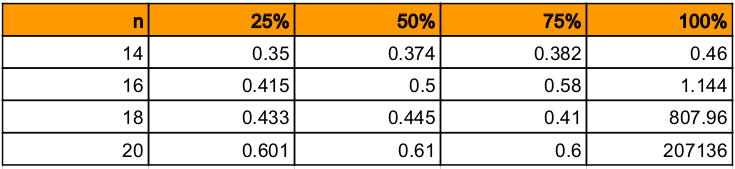
\includegraphics[scale=0.50]{graficos/tablak13.png}
		\end{center}
	\end{figure}\\

\end{document}
% Fin Ejercicio 1

\newpage
% Comienzo Ejercicio 1
\section{Heurística constructiva golosa}
\subsection{Desarrollo}
\subsubsection{Ideas preliminares}

Partiremos de la siguiente premisa: el enunciado del problema nos presenta un grafo con nodos y aristas con peso que iniciden sobre los mismos. Podemos de esta forma pensar en ``nodos con peso'': es decir, un nodo se representa con un entero que es el número con el cual se lo identifica, y un peso, que es el peso de las aristas que inciden sobre él.


\subsubsection{Explicación del algoritmo}

En primer lugar, definiremos la noción de \textit{peso\_intrapartición} ya que sera relevante a lo largo del algoritmo.
Llamaremos \textit{peso\_intrapartición} de un nodo a la suma de los pesos de las aristas que inciden sobre un él en una partición de nodos dados.
A continuación, presentamos un pseudocódigo de la función que calcula el peso\_intrapartición de un nodo en una partión, según las aristas de un grafo dado.\\
Si la partición es vacía, es decir, si el nodo va a insertarse en un subconjunto solo, como no va a haber aristas que incidan sobre él, su peso\_intrapartición será 0.\\
Caso contrario, se iterará sobre todos los nodos presentes en la partición y para cada uno, se buscará el peso de la arista entre éste y el nodo que se quiere averiguar el peso\_intrapartición y se irá sumando ese resultado. A terminar de iterar el conjunto, se tendrá el peso\_intrpartición del nodo.

Sea \textbf{conjunto} = set(int)

\begin{lstlisting}
int peso_intraparticion(int i, grafo g, conjunto particion){
	if(particion.empty){
		return 0
	} else{
		sumaPesos <- 0
		for(nodo in particion){
			sumaPesos += grafo[i][nodo]
		}
	}
	return sumaPesos
}
\end{lstlisting}

A continuación, el algoritmo constructivo goloso.\\
Describiremos la solución implementada, dividiéndola en dos etapas.

\bigskip
\begin{enumerate}
\item


\textbf{Preparación de los datos en distintas estructuras:}

Recepción del input y su posterior implementación como la matriz de adyacencias del grafo que se pasó como parámetro. Utilizamos una matriz de enteros, en el que en cada posición i:j guardamos el peso de la arista que incide sobre los nodos i y j. En caso de que dichos nodos no sean adyacentes, consideramos peso 0.

A continuación, creamos las estructuras necesarias para obtener la solución y devolver el resultado de la instancia. En el siguiente fragmento de pseodocódigo mostramos las operaciones realizadas.\\

Sea \textbf{k} = cantidad de particiones pasadas como input.\\
Sea \textbf{n} = cantidad de nodos pasados como input.\\
Sea \textbf{nodoConPeso} un struct en el que representamos un nodo según su id y su peso\_intrapartición en un conjunto determinado. Este struct cuenta con la operación de comparaciónPorPeso que justamente, compara dos nodoConPeso por su peso.\\
Sea \textbf{g} = la matriz de adyacencia formada a partir del grafo pasado como input, según los nodos y las aristas (con su respectivo peso) incidentes a cada uno de los nodos.\\
Sea \textbf{conjunto} = vector(set(int)).\\
\newpage

\begin{lstlisting}[mathescape]
particiones <- vector(conjunto) de k elementos
conjuntoNodos <- conjunto
for(nodo in n){
	inserto nodo en conjuntoNodos
}

pesos <- vector(nodoConPeso) de n elementos
for(nodo in n){
	pesos[nodo] <- nodoConPeso(nodo, peso_intraparticion(nodo, g, conjuntoNodos))
}

ordenar el vector pesos de manera creciente usando ComparacionPorPeso.
\end{lstlisting}


\textit{Particiones} representa los k conjuntos de nodos en los que podemos subdividir a los nodos. Este dato fue pasado como parámetro del problema en el input.

Insertamos en \textit{conjuntoNodos} los n nodos, o más bien, el entero que los representa para poder usar luego este conjunto para calcular el peso\_intrapartición de los nodos cuando se encuentran todos en un mismo conjunto, es decir, como se encuentran en el grafo originalmente.

Creamos un vector de n posiciones, \textit{pesos} en el que almacenaremos los  los n nodosConPeso, utilizando para cada nodo el peso\_intrapartición del nodo en el \textit{conjuntoNodos}, es decir, la suma de los pesos de las aristas (x, i), siendo x el nodo del cual queremos averiguar el peso e i un nodo de \textit{conjuntoNodos}, $\forall i \in$ \textit{conjuntoNodos}. Por último, lo ordenamos. De esta forma, los nodos quedan ordenados en el vector \textit{pesos} del más \"pesado\", es decir, aquel que su peso\_intrapartición era mayor en \textit{conjuntoNodos}.\\

\item \textbf{Alogritmo greedy:}
En esta etapa trabajamos sobre el vector \textit{pesos}. Tomaremos cada uno de los nodos guardados en él (como lo ordenamos en el paso anterior, iremos tomando desde los nodos más "pesados" hasta los más "livianos").\\
La idea subyacente será, para cada uno de los nodos tomados en orden, encontrar cuál es el conjunto del vector \textit{particiones} en el cuál el nodo tiene peso\_intrapartición mínimo.\\
Entonces, por cada uno de los nodos de \textit{pesos}, tomamos como su menorPeso (inicial) al peso\_intrapartición de ese nodo en \textit{conjuntoNodos}.\\
Luego, para cada uno de los k subconjuntos de \textit{particiones} chequeamos si el peso del nodo en la partición que se esta chequeando es menor o igual al menorPeso guardado hasta el momento. Si lo es, actualizamos el menorPeso y guardamos el subconjunto en el que fue encontrado.\\
Al terminar de chequear en los k conjuntos, tenemos el conjunto en el que un nodo alcanza su peso\_intrapartición mínimo, entonces, lo sacamos de \textit{conjuntoNodos} y lo ponemos en el nuevo subconjunto. Nótese que como al comenzar el algoritmo se calcula el menorPeso del nodo en  \textit{conjuntoNodos}, tras sacar un nodo de éste, se calcula el peso del siguiente nodo en un conjunto \textbf{sin} el nodo que fue sacado en una iteración previa.\\
\end{enumerate}

\begin{lstlisting}[mathescape]
for nodo in pesos{
	menorPeso <- peso_intraparticion(nodo, g, conjuntoNodos)
	for(l in k){
		pesoEnL <- peso_intraparticion(nodo, g, particiones[l])
		if(pesoEnL <= menorPeso){
			menorPeso <- pesoEnL
			particionElegida <- l
		}
	}
	conjuntoNodos.erase(nodo)
	particiones[particionElegida].insert(nodo)
}
\end{lstlisting}


Al terminar las n iteraciones, en el vector \textit{particiones} tenemos todos los nodos que se pasaron como input pero colocados en el conjunto en el cuál su peso\_intrapartición era el menor (en el momento en que se evaluó ese nodo).


\newpage
\subsection{Complejidad}

Para el análisis de complejidad, dividiremos nuevamente al problema en secciones como en el inciso anterior. Para comodidad del lector y facilidad de lectura, transcribiremos los fragmentos de pseudocódigo pertinentes a la demostración.
Como en el apartado anterior, describimos algunos renombres:

\noindent Sea \textbf{k} = cantidad de particiones pasadas como input.\\
Sea \textbf{n} = cantidad de nodos pasados como input.\\
Sea \textbf{nodoConPeso} un struct en el que representamos un nodo según su id y su peso\_intrapartición en un conjunto determinado. Este struct cuenta con la operación de comparaciónPorPeso que justamente, compara dos nodoConPeso por su peso.\\
Sea \textbf{g} = la matriz de adyacencia formada a partir del grafo pasado como input, según los nodos y las aristas (con su respectivo peso) incidentes a cada uno de los nodos.\\
Sea \textbf{conjunto} = vector(set(int)).\\


\textbf{\underline{Sección I-Auxiliar:} Análisis de la función peso\_intrapartición}

\begin{lstlisting}
int peso_intraparticion(int i, grafo g, conjunto particion){
	if(particion.empty){
		return 0
	} else{
		sumaPesos <- 0
		for(nodo in particion){
			sumaPesos += grafo[i][nodo]
		}
	}
	return sumaPesos
}
\end{lstlisting}

Para esta sección tenemos, en la segunda línea, el chequeo de si un set de enteros es vacío. Esto tiene complejidad $O(1)$ según la documentación de C++.\\\\
Luego, en la línea 6 iteramos sobre un set de enteros lo cual tiene una complejidad lineal sobre la cantidad de elementos del set (ya que el set de la librería de C++ está implementado sobre un ABB), por lo que n veces realizamos una asignación en una variable.\\\\
Para representar al grafo utilizamos un vector de vectores de enteros. El vector tiene n elementos, y cada vector también (ya que estamos representando al grafo en una matriz de adyacencias). De esta forma, la asignación mencionada anteriormente tiene complejidad constante, ya que es tomar el elemento ij en la matriz.\\\\
Por lo tanto, en esta sección tenemos la siguiente complejidad temporal:\\\\
$O(1)$ (Por chequear si el set es vacío y devolver 0 si ese es el caso) y $n*(O(1))$ en el caso de que el set no sea vacío y haya que iterar el set de nodos y asignar en la variable el valor de la matriz.\\\\
Finalmente, la complejidad de obtener el peso\_intrapartición de un nodo termina siendo $O(n)$.


\textbf{\underline{Sección II:} Recepción y preparación del input}

\begin{lstlisting}[mathescape]
particiones <- vector(conjunto) de k elementos
conjuntoNodos <- conjunto
for(nodo in n){
	inserto nodo en conjuntoNodos
}

pesos <- vector(nodoConPeso) de n elementos
for(nodo in n){
	pesos[nodo] <- nodoConPeso(nodo, peso_intraparticion(nodo, g, conjuntoNodos))
}

ordenar el vector pesos de manera creciente usando ComparacionPorPeso.
\end{lstlisting}


En esta sección tenemos, en la primera línea crear un vector de conjuntos. El vector tiene k elementos, y como crear un set vacío tiene complejidad constante, la complejidad de la creación del vector \textit{particiones} es lineal en k.\\\\
En la línea 2, tenemos la creación de un conjunto en el que, en las siguientes líneas insertaremos los enteros que representan a los n nodos pasados como parámetros. La creación del conjunto, como mencionamos anteriormente, es constante. La inserción es logarítimica en la cantidad de elementos del conjunto, por lo que la complejidad termina resultando $O(n*log (n))$, ya que en el peor caso, en el conjunto están todos los nodos.\\\\
En la línea 7, creamos un vector de nodoConPeso vacío y con n posiciones, y en la línea siguiente, en cada posición del vector creamos un nodoConPeso. Insertar en el vector tiene complejidad constante, ya que como tine n posiciones y no vamos a insertar más de n nodos, el vector no se va a redmiensionar. Sin embargo, la asignación del peso del nodoConPeso tiene la complejidad de calcular el peso\_intrapartición de un nodo en un set de nodos, que en el peor caso puede contenerlos a todos. De esta forma, la complejidad de las líneas 6 y 7 queda $O(n)$ (por la creación del vector de n posiciones) + $n*(O(n))$(por calcular n veces la complejidad del peso\_intrapartición de un nodo, que en el peor caso cuesta $O(n)$). Entonces, la complejidad de estas líneas es de O($n^2$) en peor caso.\\\\
Finalmente, en la línea 12 realizamos el ordenamiento, utilizando el sort de la librería stl de C++, cuya complejidad es $O(n*log (n))$, siendo n la cantidad de elementos a ordenar(en este caso, son la cantidad de nodos). Como función de comparación usamos la comparaciónPorPeso que compara el peso de dos nodoConPeso, y cuya complejidad es constante.\\\\
Entonces, para esta sección, la complejidad temporal es:\\\\
$k + O(n*log(n))+O(n)+ O(n^2)+O(n*log(n)) = k + 2*O(n*log(n)) + O(n) + O(n^2) = k +  O(n^2)$\\

\textbf{\underline{Sección 3:} Algoritmo greedy}

\begin{lstlisting}[mathescape]
for nodo in pesos{
	menorPeso <- peso_intraparticion(nodo, g, conjuntoNodos)
	for(l in k){
		pesoEnL <- peso_intraparticion(nodo, g, particiones[l])
		if(pesoEnL <= menorPeso){
			menorPeso <- pesoEnL
			particionElegida <- l
		}
	}
	conjuntoNodos.erase(nodo)
	particiones[particionElegida].insert(nodo)
}
\end{lstlisting}

Para la última sección del algoritmo, tenemos, en la primer línea, la iteración sobre un vector de n elementos.\\\\
En la línea 2, tenemos la asignación en una variable del peso\_intrapartición de un nodo, lo cual como vimos en la Sección I tiene complejidad lineal sobre la cantidad de nodos.\\
Luego, k veces obtener el peso\_intrapartición de un nodo en una partición, lo que en peor caso tiene complejidad lineal, como mencionamos ya previamente. Después de esta asignación, relizamos en las líneas subsiguientes (5, 6, 7) operaciones de complejidad constante, tales como comparaciones entre enteros y asignación en variables. Entonces entre las líneas 4 y 7 tenemos una complejidad asintótica de $O(n) + 3*O(1) = O(n)$.\\\\
Por último realizamos en las últimas dos líneas las operaciones erase e insert de set, que según la documentación de C++ tienen complejidad $O(log(n))$ ambas.\\\\
De esta forma, la complejidad para esta sección queda:\\

$n*[O(n)+k*(O(n))+O(log(n))+O(log(n)] = n*[O(n)+k*(O(n) + 2*O(log(n)))] = $ \\\\
$n*O(n) + k*n*O(n) = O(n^2) + O(k*n^2) = O(k*n^2)$\\


\newpage
\textbf{\underline{Complejidad final del algoritmo:}}\\

$k +  O(n^2)$ (por la sección II) $+ O(k*n^2)$ (por la sección III) $=  O(k*n^2)$\\

\subsection{Análisis soluciones no óptimas}

El algoritmo greedy no dará soluciones óptimas cuando ponga en un conjunto un nodo para el que, en el momento en el que se realizó dicha decisión, ese conjunto era el que hacía que aportara menor peso, pero que en realidad, colocarlo en otro llevara a una solución mejor.\\
En otras palabras, la heurística golosa toma una decisión basándose en un criterio en cada iteración, sin tener en cuenta si tomar una decisión distinta lo hubiera llevado a alcanzar una mejor solución.\\
En el caso de nuestro algoritmo, ese criterio es:\\


" Tomar el nodo que mayor peso\_intrapartición tenga en \textit{conjuntoNodos} y ponerlo en el conjunto para el que su peso\_intrapartición sea menor (o igual, si no hay uno menor). En caso de que haya dos o más conjuntos en los que el nodo podría ir -basándonos en este criterio-, por cómo está implementado el algoritmo, se elige el último en el que se consultó el peso\_intrapartición del nodo"


A continuación, describiremos una instancia para la cual esta heurística golosa no ofrece una solución óptima.\\

Sea la siguiente instancia:\\

	\begin{tabular}{| l | l | l |}
	\hline
	5 & 5 & 2\\
	3 & 1 & 300\\
	1 & 4 & 1\\
	1 & 2 & 1000\\
	4 & 2 & 10\\
	4 & 5 & 1150\\

	\hline
	\end{tabular}

Veamos como funciona el algoritmo en la instancia planteada. \\

\begin{enumerate}
\item Pone todos los nodos en un conjunto inicial, \textit{conjuntoNodos}.

\textit{conjuntoNodos}: \{1, 2, 3, 4, 5\}

\item Calcula el peso de los nodos en \textit{conjuntoNodos} y a partir de este peso, los ordena en el vector \textit{pesos}. El peso inicial de los nodos en esta instancia es:

1 = 1301\\
2 = 1010\\
3 = 300\\
4 = 1161\\
5 = 1150\\

Entonces, el vector \textit{pesos} queda: [1, 4, 5, 2, 3] y los nodos serán sacados del \textit{conjuntoNodos} en ese orden.\\

\item Recorre las k particiones y para cada uno de los nodos chequea si el peso del nodo en \textit{conjuntoNodos} es menor o igual que en la partición i-ésima. Si lo es, guarda esa partición como la elegida para ubicar al nodo. Cuando termina de iterar las k particiones, saca el nodo de \textit{conjuntoNodos} y lo pone en la partición elegida.
\end{enumerate}


Veamos para cada nodo como se elige la partición en la cuál ubicarlo.

\begin{enumerate}

\item
Peso de 1 en \textit{conjuntoNodos} en el que estan los nodos \{1, 2, 3, 4, 5\}: 1301\\
Peso de 1 en partición 1 en la que estan los nodos \{\}: 0 \\
Peso en 1 en partición 2 en la que estan los nodos \{\}: 0 \\

Saca el 1 de \textit{conjuntoNodos} y lo pone en la partición 2\\

\item
Peso de 4 en \textit{conjuntoNodos} en el que estan los nodos \{2, 3, 4, 5\}: 1160\\
Peso de 4 en partición 1 en la que estan los nodos \{\}: 0 \\
Peso en 4 en partición 2 en la que estan los nodos \{1\}: 1 \\

Saca el 4 de \textit{conjuntoNodos} y lo pone en la partición 1\\

\item
Peso de 5 en \textit{conjuntoNodos} en el que estan los nodos \{2, 3, 5\}: 0\\
Peso de 5 en partición 1 en la que estan los nodos \{4\}: 1150 \\
Peso en 5 en partición 2 en la que estan los nodos \{1\}: 0 \\

Saca el 5 de \textit{conjuntoNodos} y lo pone en la partición 2\\

\item
Peso de 2 en \textit{conjuntoNodos} en el que estan los nodos \{2, 3\}: 0\\
Peso de 2 en partición 1 en la que estan los nodos \{4\}: 10 \\
Peso en 2 en partición 2 en la que estan los nodos \{1, 5\}: 1000 \\

Saca el 2 de \textit{conjuntoNodos} y lo pone en la partición 1\\

\item
Peso de 3 en \textit{conjuntoNodos} en el que estan los nodos \{3\}: 0\\
Peso de 3 en partición 1 en la que estan los nodos \{4, 2\}: 10 \\
Peso en 3 en partición 2 en la que estan los nodos \{1, 5\}: 1000 \\

Saca el 3 de \textit{conjuntoNodos} y lo pone en la partición 1\\
\end{enumerate}

\noindent Finalmente los nodos quedan ubicados de la siguiente manera.\\
Partición 1: \{4, 2, 3\}\\
Partición 2: \{1, 5\}\\
Suma de los pesos de las particiones = 10.\\

\noindent Sin embargo, una partición óptima era ubicar los nodos de esta manera\\
Partición 1: \{2, 3, 5\}\\
Partición 2: \{1, 4\}\\
Suma de los pesos de las particiones = 1.\\

En el paso 2, el peso\_intrapartición del nodo 4 es 0 en el conjunto 1 y 1 en el conjunto 2. Si en este paso, hubiera decidido ponerlo sin seguir el criterio, y se hubiera puesto en el conjunto 2

\begin{enumerate}
\item
Peso de 5 en \textit{conjuntoNodos} en el que estan los nodos \{2, 3, 5\}: 0\\
Peso de 5 en partición 1 en la que estan los nodos \{\}: 0 \\
Peso en 5 en partición 2 en la que estan los nodos \{1,4\}: 1150 \\

Saca el 5 de \textit{conjuntoNodos} y lo pone en la partición 1\\

\item
Peso de 2 en \textit{conjuntoNodos} en el que estan los nodos \{2, 3\}: 0\\
Peso de 2 en partición 1 en la que estan los nodos \{5\}: 0 \\
Peso en 2 en partición 2 en la que estan los nodos \{1, 4\}: 1010 \\

Saca el 2 de \textit{conjuntoNodos} y lo pone en la partición 1\\

\item
Peso de 3 en \textit{conjuntoNodos} en el que estan los nodos \{3\}: 0\\
Peso de 3 en partición 1 en la que estan los nodos \{5, 2\}: 0 \\
Peso en 3 en partición 2 en la que estan los nodos \{1, 4\}: 300 \\

Saca el 3 de \textit{conjuntoNodos} y lo pone en la partición 1\\
\end{enumerate}


\noindent De esta forma, los nodos quedan ubicados de esta forma, dando una solución óptima al problema:\\
Partición 1: \{2, 3, 5\}\\
Partición 2: \{1, 4\}\\
Suma de los pesos de las particiones = 1.\\


Ahora bien, se puede ver que incrementando el peso de la arista (4,2) que es la que el algoritmo greedy decide poner en una partición que lo aleja de la solución óptima, podemos empeorar la solución que brindamos. Por ejemplo, si el peso fuera 100, la solución brindada por el algoritmo greedy daría una suma de pesos de particiones de 100 mientras que la solución óptima seguiría siendo de 1.\\
Hay que tener en cuenta que tampoco podemos incrementar indiscriminadamente los pesos de las aristas sin que se modifique sustancialmente el grafo sobre el cual corremos el algoritmo, y de esta forma, cambien las decisiones tomadas en cada instancia. Sin embargo, como mostramos anteriormente, sí podemos modificar las instancias de manera tal que empeore la solución otorgada por el algoritmo greedy y la solución del algoritmo exacto no se modifique.\\

Concluímos entonces que evaluando en cada iteración dónde debe ir un nodo en función del estado actual de las particiones no nos lleva indefectiblemente a una solución óptima, ya que puede pasar, como se ve en el ejemplo, que convenga tomar una decisión que nos aleje del óptimo en una iteración, pero que finalmente, lleve a la solución óptima cuando el total de los nodos queda ubicado en las particiones. De todas formas, el algoritmo constructivo goloso termina brindando una solución aproximada y relativamente rápida para grafos de un tamaño considerable, tal como veremos en la sección siguiente.\\


\subsection{Experimentación}

Para el proceso de experimentación del problema se plantearon distintas pruebas para corroborar que el algoritmo propuesto funcionara correctamente, y que la cota de complejidad encontrada y justificada en la sección anterior, se cumpliera en la práctica.

\noindent Dado que el CPU de la computadora utilizada para tomar los tiempos no está atendiendo únicamente a nuestro proceso, realizar una sola vez cada prueba podría darnos valores que no son cercanos a los reales. Por lo tanto, para minimizar este margen de error, a cada prueba se la hizo ejecutar un total de 10 veces, y se tomó el mejor valor, es decir, el menor tiempo de ejecución obtenido. Notar que, tomar el mejor valor no es una mala decisión, ya que cuanto más chico sea el valor, más cerca estamos del valor real de tiempo que toma el algoritmo para una instancia dada.\\

\noindent En cada prueba, se tomaron métricas para la posterior evaluación del algoritmo en la práctica. Vale aclarar que la medición no contempla tiempos de recepción y salida de datos, sino que contempla:\\

\noindent \begin{enumerate}
\item Preparación del input en las estructuras mencionadas en los apartados anteriores.
\item El algoritmo constructivo goloso que da la solución al problema.\\
\end{enumerate}

\noindent Para el testeo, se diseñó un generador de instancias aleatorias que toma como parámetros los nodos y aristas del grafo, y la cantidad de particiones sobre las cuales se quiere k-particionar al grafo.\\

\noindent Con este programa pudimos evaluar cuánto tiempo de ejecución toma nuestro algoritmo para distintas instancias aleatorias del problema.\\

\noindent Para todos los casos, se eligió una precisión de hasta 0,0001 ms (milisegundos). De ser menor, la tomamos como 0.\\

\noindent Finalmente, el proceso de testing es:\\

\noindent \begin{enumerate}
\item Generación de instancia aleatoria, según parámetros prefijados.
\item Ejecución de dicha instancia 10 veces, tomando el mejor tiempo obtenido.
\item Repetición de los items 1 y 2 otras 14 veces y obtención del tiempo promedio.
\end{enumerate}

\noindent Con esta metodología de experimentación, realizamos dos tipos de pruebas:\\

\noindent \begin{itemize}
\item Variando la cantidad de nodos, manteniendo en proporción constante relativa a los nodos la cantidad de aristas y dejando fija la cantidad de particiones.
\item Variando la cantidad de particiones y dejando fija la cantidad de nodos y aristas.\\
\end{itemize}

\noindent A continuación, describiremos las particularidades de cada tipo de prueba.

\subsubsection{Experimentación variando la cantidad de nodos}

Para este set de experimentos, variamos n (la cantidad de nodos) de 50 a 500 (incrementando de a 50 nodos) y mantuvimos constante la cantidad de aristas, relativas a la cantidad de nodos, en una proporción $m = n*4$, ya que nos pareció una cantidad interesante para que el grafo tuviera suficientes conexiones.\\ La cantidad de particiones se mantuvo fija en 10.
A partir de los resultados obtenidos, observamos a que el gráfico resultante se condice con la complejidad calculada teóricamente, siendo la variación en n cuadrática.\\
A continuación, mostraremos la tabla con los valores obtenidos, y los gráficos representando los tiempos de ejecución y la estimación de la complejidad del algoritmo.

\noindent \textit{Aclaración I : Para una mejor representación, los valores de tiempos obtenidos y mostrados en las tablas fueron multiplicados por 1000 para graficarlos, por lo tanto los tiempos están expresados en nanosegundos.}\\

\noindent \textit{Aclaración II: Por simplicidad, nos referiremos como en el resto del informe a:}\\

\noindent \begin{itemize}
\item \textbf{n} = cantidad de nodos.
\item \textbf{m} = cantidad de aristas.
\item \textbf{k} = cantidad de particiones.
\end{itemize}

\begin{center}
	\begin{tabular}{| l | l | l | l |}
	\hline
	n & tiempo & $tiempo/n$ & $tiempo/n^2$\\ \hline
	50 & 2,6509 & 0,053018 & 0,00106036\\
	100 & 10,6189 & 0,106189 & 0,00106189\\
	150 & 24,6199 & 0,1641326667 & 0,0010942178\\
	200	& 64,0654 & 0,320327 & 0,001601635\\
	250 & 99,0569 & 0,3962276 & 0,0015849104\\
	300 & 144,893 & 0,4829766667 & 0,0016099222\\
	350 & 195,9567 & 0,5598762857 & 0,0015996465\\
	400 & 257,1133 & 0,64278325 & 0,0016069581\\
	450 & 322,2716 & 0,7161591111 & 0,0015914647\\
	500	& 396,8685 & 0,793737 & 0,001587474\\
	\hline
	\end{tabular}
\end{center}

En el primer gráfico, vemos como la gráfica correspondiente a ejecutar el algoritmo como se describió anteriormente, tiene una forma cuadrática.

\begin{figure}[h]
	\begin{center}
	   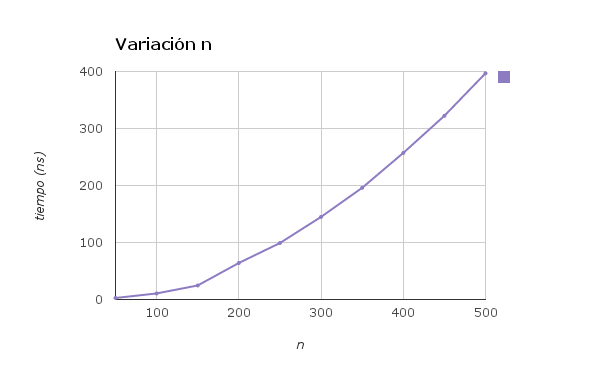
\includegraphics[scale=0.50]{ejercicio3/n.png}
	\end{center}
\end{figure}

En el segundo gráfico, realizamos para cada punto la división del tiempo sobre n. Como estimamos que la curva del gráfico anterior era cuadrática, esta debería ser lineal. Por el gráfico, podemos observar que sigue la tendencia esperada.

\begin{figure}[h]
	\begin{center}
	   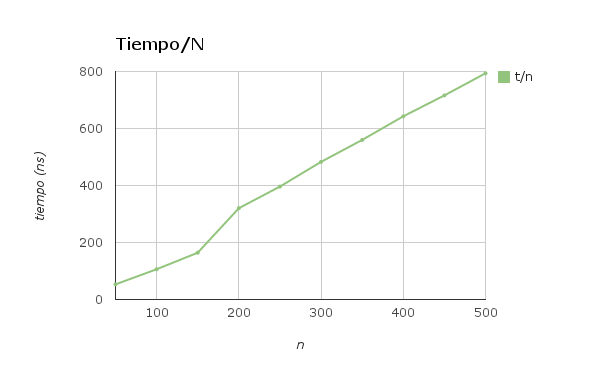
\includegraphics[scale=0.50]{ejercicio3/n_sobren.png}
	\end{center}
\end{figure}

Por último, en el tercer gráfico, realizamos la división de cada punto por el tiempo sobre $n^2$. Como esperábamos, la función resultante es constante.

\begin{figure}[h]
	\begin{center}
	   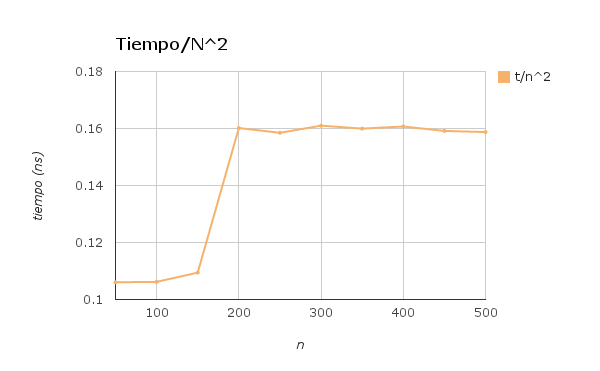
\includegraphics[scale=0.50]{ejercicio3/n_sobren2.png}
	\end{center}
\end{figure}

\subsubsection{Experimentación variando la cantidad de nodos}

Para este set de experimentos, variamos k (la cantidad de particiones) de 10 a 150 (incrementando de k de a 10) y mantuvimos constante la cantidad de nodos y aristas. Fijamos los nodos en 100 y las aristas en 150.
A partir de los resultados obtenidos, observamos a que el gráfico resultante se condice con la complejidad calculada teóricamente, siendo la variación en k lineal.\\
A continuación, mostraremos la tabla con los valores obtenidos, y los gráficos representando los tiempos de ejecución y la estimación de la complejidad del algoritmo.

\begin{center}
	\begin{tabular}{| l | l | l |}
	\hline
	k & tiempo & $tiempo/k$ \\ \hline
	10 & 2,342375 & 0,2342375\\
	20 & 2,426375 & 0,12131875\\
	30 & 2,508025 & 0,08360083333\\
	40	& 2,552925 & 0,063823125 \\
	50 & 2,674425 & 0,0534885 \\
	60 & 2,71455 & 0,0452425\\
	70 & 2,8401 & 0,04057285714\\
	80 & 2,861375 & 0,0357671875\\
	90 & 2,94165 & 0,032685\\
	100	& 2,968175 & 0,02968175\\
	110	& 3,029625 & 0,02754204545\\
	120	& 3,112725 & 0,025939375\\
	130	& 3,1983 & 0,02460230769\\
	140	& 3,272575 & 0,02337553571\\
	150	& 3,31775 & 0,02211833333\\
	\hline
	\end{tabular}
\end{center}

En el primer gráfico, vemos como la variación del tiempo a medida que se incrementa el número de particiones es lineal en k.

\begin{figure}[h]
	\begin{center}
	   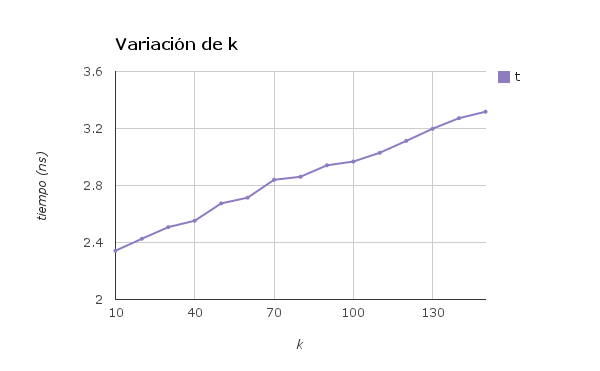
\includegraphics[scale=0.50]{ejercicio3/k.png}
	\end{center}
\end{figure}

En este segundo gráfico, podemos corroborarlo, ya que al dividir cada punto por k, obtenemos una gráfica constante.

\begin{figure}[h]
	\begin{center}
	   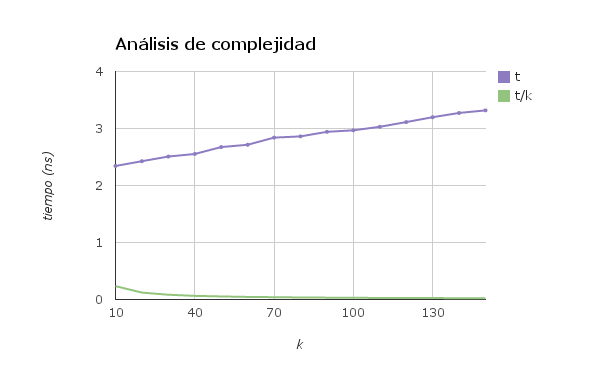
\includegraphics[scale=0.50]{ejercicio3/k_sobrek.png}
	\end{center}
\end{figure}



Aunque estos experimentos no bastan para mostrar la correctitud de la demostración de complejidad realizada previamente, los resultados obtenidos parecen indicar que nuestras estimaciones teóricas eran correctas y la complejidad del algoritmo constructivo goloso es $O(k*n^2)$

% Fin Ejercicio 1

\newpage
% Comienzo Ejercicio 1
\documentclass[10pt,a4paper]{article}
\usepackage[utf8]{inputenc} % para poder usar tildes en archivos UTF-8
\usepackage[spanish]{babel} % para que comandos como \today den el resultado en castellano
\usepackage{fullpage} %small margins
\usepackage[parfill]{parskip} %genera saltos entre parrafos
\usepackage{color}
\definecolor{gray}{gray}{0.35}
\usepackage{listings}
\usepackage{enumitem}
\usepackage{amsmath} %big brackets
\lstset{
    numbers=left,
    breaklines=true,
    tabsize=2,
    basicstyle=\ttfamily\color{gray},
}
\setlength{\parindent}{8pt}
\usepackage{mathtools}
\usepackage[margin=50pt]{geometry}
\usepackage{amsfonts}
\usepackage{flafter}
\usepackage{multicol}
\usepackage{subcaption}

\begin{document}

\section{Heurística de búsqueda local}
\subsection{Introduccion}

¿Qué es una \textbf{heurística de búsqueda local}? Una heurística de busqueda local, como su nombre indica, es un \textbf{procedimiento que busca, partiendo de una solución inicial $s$, una que sea mejor} que $s$ a través de "vecinos".

¿Qué son los vecinos de una solución? \textbf{Los vecinos de \boldmath{$s$}, denominados \boldmath{$N(s)$}} siendo $s$ una solución factible al problema, son aquellos que puedo \textbf{obtener realizando una modificación a \boldmath{$s$}}. Esa modificación es ad hoc al problema en sí, y, de hecho, la vecindad de una solución está definida por esa modificación. Por ejemplo, en k-PMP, si la vecindad está definida por tomar un nodo $v$ de un conjunto y colocarlo en otro conjunto, una solución $s$ tiene $s' \in N(s) \Leftrightarrow$ puedo obtener a $s'$ tomando un nodo $v$ de un conjunto y colocarlo en otro. Para esta vecindad, ocurre que $s \in N(s')$ ya que basta con colocar $v$ en su conjunto original.

¿Mejorar en cuánto a qué? Los problemas de \textbf{optimización combinatoria}, como el que es analizado en este trabajo práctico, son los cuáles se busca \textbf{optimizar una función \boldmath{$f:S\rightarrow \mathbb{R}$}}, donde $S$ es el conjunto de soluciones factibles para su correspondiente instancia $I$. La función $f$ para este problema es $f(s) =$ peso de solución $s$, con $s \in S$ para la instancia $I$ asociada. Por ende, \textbf{una solución \boldmath{$s'$} es mejor que una solución \boldmath{$s \Leftrightarrow f(s') < f(s)$}}. \textbf{La factibilidad de una solución está atada a reglas del problema}. Por ejemplo, en el k-PMP, una solución no puede distribuir menos nodos, en la partición, de los que tiene el grafo de entrada, tampoco podría describir una partición $P$ tal que $|P| > k$, etc.

¿Que nos detiene de \textbf{obtener la mejor solución}? \textbf{Encontrar la óptima es, efectivamente, resolver el problema}. La necesidad de tener heurísticas, de cualquier tipo, surge de \textbf{no conocer algoritmos que resuelvan la problemática en tiempo polinomial}, como es el caso del k-PMP. Por ende, buscamos algoritmos que nos permitan obtener soluciones ``buenas'' en un tiempo más razonable.

En particular, ¿por qué existen las busquedas locales? Dichas búsquedas proveen un servicio de \textbf{mejoramiento a otros algoritmos que generen soluciones}. Supongamos que una instancia $I$ fue puesta a través de un algoritmo heurístico goloso $HG$. Si esa instancia $I$ era particularmente mala para dicha heurística, la solución obtenida podría estar muy alejada de la óptima, que es lo que queremos tratar de evitar. Una buena idea es someter esa solución a un algoritmo de búsqueda local $HBL$ que atente a mejorarla. Al ser un algoritmo distinto, explora distintas posibilidades que la $HG$ no pudo ver.

¿\textbf{Siempre se puede llegar a una solución óptima de esta manera}? No siempre. \textbf{Si fuese así, tendríamos un algoritmo que resuelva el problema en tiempos razonables}. Por tiempos razonables nos referimos a tiempos no exponenciales, no podemos asegurar que siempre sean polinomiales ya que no toda heurística tiene una cota polinomial definida. Hasta puede ocurrir que para ciertas instancias sea imposible alcanzar el óptimo, por como fue definida vecindad, por como es la solución, o una mezcla de ambas. Hay heurísticas, denomidadas aproximadas, que tienen cotas de cuán mala puede ser la solución encontrada por dicho algoritmo. Sabiendo eso, si la cota no es muy holgada, combinar esa heurística con una de búsqueda local tendría altas probabilidades de generar muy buenas, o inclusive óptimas, soluciones. Pero, de nuevo, ni siquiera en esos casos podemos asegurar que siempre vamos a encontrar una óptima. \textbf{Esta es la razón por la cuál se denominan busquedas \textit{locales}}. \textbf{Buscan la mejor solucion, denominada óptimo local, en un conjunto \boldmath{$S'$} de soluciones tal que \boldmath{$S' \subseteq S$}, donde \boldmath{$S$} es el conjunto total de soluciones}, que depende de la solución inicial, de la vecindad planteada y de la instancia.

Habiendo dicho esto, \textbf{el procedimiento de la heurística de busqueda local es, dada una solución $s$, elegir el óptimo local $o$ dentro del conjunto $S' \subseteq S$ que forma la vecindad}. Entonces, esta solución $o$ es alguna una tal que $o \in S'$ y $f(o) \leq f(s')$, $\forall s' \in S'$, donde $f$ es la función a optimizar.

\newpage
\subsection{Busqueda Local 1}
\subsubsection{Desarrollo}
\noindent \textbf{\underline{Explicación de vecindad de la búsqueda local 1}}

El modo en que este algoritmo de búsqueda local va a operar es \textbf{revisando todos los vecinos de una solución y eligiendo el mejor}. Elegimos en el conjunto $S' = \left\{s\right\} \cup N(s)$ el óptimo local. Para toda solución $s$, la vecindad está definida por la siguiente función:

\textbf{\boldmath{$N1(s) =$} intercambiar un nodo \boldmath{$v$} en un conjunto, por otro nodo \boldmath{$u$} en otro conjunto distinto dentro la partición.}

En una solución $s$ genérica:

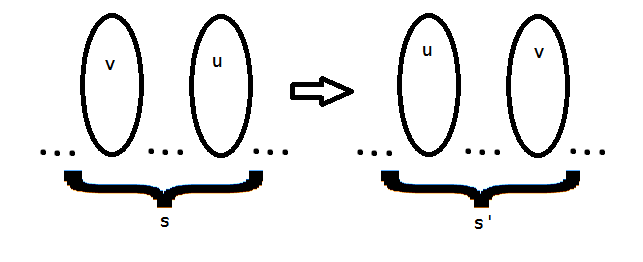
\includegraphics[scale=.75]{Vecindad1.png}

El tamaño de la vecindad depende de cuántos nodos puedo intercambiar, dejando de lado los nodos que estén en un mismo conjunto, ya que intercambiar 2 nodos dentro de un mismo conjunto deja el peso intrapartición intacto, por ende dejando el peso total intacto. En peor caso, en cuánto a cantidad de intercambios, podría pasar que todos los nodos estén en conjuntos distintos, por ende teniendo $(n-1)$ intercambios posibles para cada vértice, lo cuál genera un total $n*(n-1)$ posibles intercambios. Entonces, \textbf{para toda solución \boldmath{$s$}, \boldmath{$|N1(s)| \in O(n*(n-1)) = O(n^2)$}}. Esto nos dice que, \textbf{como mínimo, en peor caso, la función de complejidad temporal de dicho algoritmo debe ser de orden cuadrático en \boldmath{$n$} ya que esa es la cantidad de vecinos, como máximo, que podría tener una solución} y el algoritmo explora toda la vecindad.

\noindent \textbf{\underline{Pseudo código búsqueda local 1}}

\begin{lstlisting}
Solucion BusquedaLocal1(Grafo G = {v_1 ... v_n}, X), int k, Solucion s)
	Particion particion_actual = particion generada por s
	Particion mejor_particion = particion_actual
	para todo nodo v_i con i desde 1 a n:
		para todo nodo v_j con j desde 1 a n:
			si v_i esta en un conjunto distinto al v_j:
				colocar v_i en el conjunto donde se encuentra v_j dentro de la particion_actual
				colocar v_j en el conjunto donde se encontraba v_i dentro de la particion_actual
				si el peso total disminuyo:
					mejor_particion = particion_actual
				coloco v_i en su conjunto original dentro de la particion actual
				coloco v_j en su conjunto original dentro de la particion actual
				fin si
			fin si
		fin para
	fin para
	
	Solucion mejor_solucion = solucion asociada a la mejor_particion
	return mejor_solucion
\end{lstlisting}

Detalles a notar:
\begin{itemize}
\item No hace falta preguntar si $v_i \neq v_j$ ya que si están en conjuntos distintos, lo son.
\end{itemize}

\subsubsection{Complejidad}
\noindent \textbf{\underline{Comentarios preliminares}}
\begin{itemize}
\item Decidimos utilizar el código fuente para el cálculo de complejidad ya que brinda un cálculo más preciso y sin ambiguedades. Consideramos la línea 1 de un algoritmo como la línea donde, en el código fuente, se encuentra el return type, la declararción y los parámetros de una función.
\item Las estructuras utilizadas en el código son set y vector, ambas de la STL de c++.
\item Definimos \textit{Grafo} como vector\textless vector\textless float\textgreater \textgreater, \textit{Solución} como vector\textless int\textgreater, \textit{Conjunto} como set\textless int\textgreater y \textit{Partición} como vector\textless Conjunto\textgreater .
\end{itemize}

\noindent \textbf{\underline{La clase BusquedaLocal1}}

Decidimos colocar la heurística dentro de una clase llamada BusquedaLocal1 que consta de:

\textbf{Miembros privados de la clase}
\begin{itemize}
\item \textit{Solución solución\_inicial}: Contiene una copia de la solución a ser mejorada por la heurística.
\item \textit{Solución mejor\_vecino}: Contiene una copia del resultado de la heurística aplicada a la solución\_inicial o una copia de la solución\_inicial.
\item \textit{float peso\_mejor\_vecino}: Contiene el peso de mejor\_vecino si es que se usó previamente la función \textit{resolver}.
\end{itemize}

\textbf{Funciones relevantes públicas de la clase}
\begin{itemize}
\item \textit{Constructor BusquedaLocal1(const Solución}\& \textit{solución)}: Constructor que toma una solución como parametro y crea un objeto de la clase \textit{BusquedaLocal1} copiando la solución pasada como parámetro a \textit{solución\_inicia}l y a \textit{mejor\_vecino}. Operación que toma $O(n)$ dado que es copiar un vector de ints de tamaño $n$, y copiar un int tiene complejidad $O(1)$.
\item \textit{Solución resolver(const Grafo}\& \textit{grafo, int k, int n)}: Función que aplica la heurística de búsqueda local 1 a \textit{solución\_inicial}, almacenando el resultado en \textit{mejor\_vecino} y devolviéndolo. Complejidad analizada más abajo. \textbf{Esta función corresponde al pseudo código de la busqueda local 1 hecho más arriba.}
\item \textit{float getPeso()}: Función que devuelve peso\_mejor\_vecino. Complejidad $O(1)$.
\end{itemize}

\noindent \textbf{\underline{Complejidad algoritomo de BusquedaLocal1::resolver}}

\begin{itemize}
\item Líneas 2 - 3: 2 copias de objetos \textit{Partición}. Copiar un \textit{Conjunto} tiene complejidad $O(n)$, ya que en peor caso puede contener a todos los vértices, y hay $k$ conjuntos, por ende la complejidad es $O(2(n*k)) = O(n*k)$.
\item Líneas 3 - 18: \textit{For} que itera sobre la cantidad de nodos $\Rightarrow O(n * cuerpoFor1) = O(n^4 * k)$.
\item $cuerpoFor1$:
\begin{itemize}
\item Líneas 5 - 17: \textit{For} que itera sobre la cantidad de nodos $\Rightarrow O(n * cuerpoFor2) = O(n*n^2*k) = O(n^3 * k)$.
\item $cuerpoFor2$: 
\begin{itemize}
\item Línea 9: Complejidad de \textit{swapear\_nodos} $\in O(log(n))$ (Ver Complejidad Algoritmos Usados).
\item Línea 10: Compejidad de \textit{peso\_de\_partición} $\in O(n^2*k)$ (Ver Complejidad Algoritmos Usados).
\item Línea 11: Copia de una \textit{Partición} $\in O(n*k)$.
\item Línea 15: Complejidad de \textit{swapear\_nodos} $\in O(log(n))$ (Ver Complejidad Algoritmos Usados).
\end{itemize}
\item Complejidad $cuerpoFor2$ $\in O(n^2*k + n*k + log(n)) = O(n^2*k)$, por propiedades de la función $O$.
\end{itemize}
\item Complejidad $cuerpoFor1$ $O(1 + n^2*k) = O(n^3 * k)$, por propiedades de la función $O$.
\item Línea 19: Copiar un float $O(1)$ y Complejidad de \textit{peso\_de\_partición} $\in O(n^2*k)$ (Ver Complejidad Algoritmos Usados) $\Rightarrow \in O(n^2*k)$.
\item Línea 20: Copiar una \textit{Solución} tiene complejidad $O(n)$ y Complejidad de \textit{convertir\_particion\_en\_solucion} $\in O(n*k)$ (Ver Complejidad Algoritmos Usados) $\Rightarrow \in O(n + n*k) = O(n*k)$.
\item Línea 21: Devolver una \textit{Solución} por copia tiene complejidad $O(n)$.
\end{itemize}

\noindent \underline{Complejidad Total}: $O(n*k + n^4*k) = O(n^4*k)$ la cuál es pseudo-polinomial en el tamaño de la entrada.

Un pequeño análisis más en detalle de la complejidad nos muestra que lo que habíamos mencionado del tamaño de la vecindad es cierto. $O(n^3*k) = O((n^2)*(n^2*k))$, donde $O(n^2)$ es el costo de recorrer los vecinos y $O(n^2*k)$ es el costo de ``armar'' y obtener el valor de $f$, la función a optimizar, de cada vecino.

\textbf{\underline{Explicación y Complejidad Algoritmos Usados}}

\begin{itemize}
\item \textit{void swapear\_nodos(int nodo\_i, int conjunto\_nodo\_i, int nodo\_j, int conjunto\_nodo\_j, Partición}\& \textit{partición\_actual)}:
\begin{itemize}
\item Función que, dados los parámetros, toma el \textit{nodo\_i} y lo coloca en el \textit{conjunto\_nodo\_j}, y luego toma el \textit{nodo\_j} y lo coloca en el \textit{conjunto\_nodo\_j}.

\item Consta de 2 llamados de función de \textit{set::erase}, que tiene complejidad $O(log(n))$, y 2 llamados de función \textit{set::insert}, que también posee complejidad $O(log(n))$, con $n$ la cantidad de elementos del \textit{set}\newline $\Rightarrow \in O(4*log(n)) = O(log(n))$.
\end{itemize}
\item \textit{float peso\_de\_particion(Partición}\& \textit{partición, int k, Grafo}\& \textit{grafo))}:
\begin{itemize}
\item Función que, dado el \textit{Grafo} correspondiente, devuelve el peso total de la \textit{Partición} pasada como parámetro.
\item Consta de un \textit{For} que itera sobre $k$ donde cada iteración tiene un \textit{For} que itera sobre el tamaño del \textit{Conjunto}, denominado $n$, con un ciclo dentro que itera sobre el tamaño del conjunto, realizando operaciones con costo temporal $O(1)$ $\Rightarrow$ la complejidad de la función es $O(k*n*n*1) = O(n^2*k)$.
\end{itemize}
\item \textit{Solución convertir\_particion\_en\_solucion(Partición}\& \textit{partición, int k}):
\begin{itemize}
\item Función que transforma una \textit{Partición} en una \textit{Solución} válida.
\item Consta de un \textit{For} que itera tantas veces como $k$ que contiene otro \textit{For} que itera sobre $n$, la cantidad de elementos del \textit{Conjunto}, realizando operaciones de complejidad constante $\Rightarrow \in O(n*k)$.
\end{itemize}
\end{itemize}

\textbf{\underline{Costo total de aplicar la heurística sobre una solución}}

\begin{itemize}
\item Tomar el input (no se tiene en cuenta en el cálculo de Complejidad).
\item Creación del objeto \textit{BusquedaLocal1} con la solución a mejorar $\in O(n)$.
\item Llamado a \textit{BusquedaLocal1::resolver} sobre ese objeto $\in O(n^4*k)$.
\end{itemize}

\underline{Complejidad Total}: $O(n^4*k)$.

\newpage
\subsection{Busqueda Local 2}
\subsubsection{Desarrollo}
\noindent \textbf{\underline{Explicación de vecindad de la búsqueda local 2}}

El modo en que este algoritmo de búsqueda local va a operar es \textbf{revisando todos los vecinos de una solución y eligiendo el mejor}. Elegimos en el conjunto $S' = \left\{s\right\} \cup N(s)$ el óptimo local. Para toda solución $s$, la vecindad está definida por la siguiente función:

\textbf{\boldmath{$N2(s) =$ colocar un nodo $v$ en un conjunto distinto al que pertenece dentro de la partición.}}

En una solución $s$ genérica:

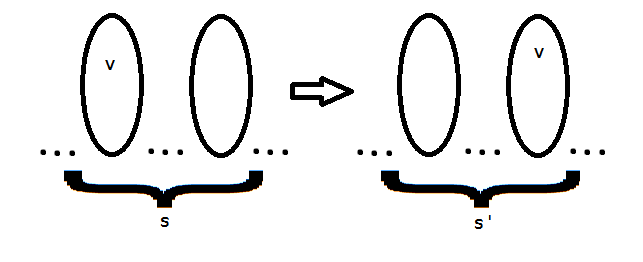
\includegraphics[scale=.75]{Vecindad2.png}

El tamaño de esta vecindad depende de en cuántos conjuntos distintos dentro de la partición puedo colocar a un vértice, y eso es siempre $(k-1)$, todos los conjuntos menos el mismo al que pertenece. Esto es cierto para todo vértice, \textbf{\boldmath{entonces para toda solución $s$ se cumple que $|N2(s)| = O(n*(k-1)) = O(n*k)$}}. Como para la anterior búsqueda local, se debe cumplir que el \textbf{\boldmath{algoritmo, como mínimo, perteneza a $O(n*k)$ dado que el algoritmo revisa toda la vecindad en busca del mejor vecino}}.

\noindent \textbf{\underline{Pseudo código de la búsqueda local 2}}

\begin{lstlisting}
Solucion BusquedaLocal1(Grafo G = {v_1 ... v_n}, X), int k, Solucion s)
	Particion particion_actual = particion generada por s
	Particion mejor_particion = particion_actual
	para todo nodo v_i con i desde 1 a n:
		para todo conjunto c_j desde 1 hasta k:
			si el nodo v_i no pertenece al conjunto c_j
				quitar v_i de su conjunto actual
				colocar v_i en el conjunto c_j
				si el peso total disminuyo:
					mejor_particion = particion_actual
				quitar v_i de c_j
				colocar v_i en su conjunto original correspondiente
				fin si
			fin si
		fin para
	fin para
	
	Solucion mejor_solucion = solucion asociada a la mejor_particion
	return mejor_solucion
\end{lstlisting}

\subsubsection{Complejidad}

\noindent \textbf{\underline{Comentarios preliminares}}
\begin{itemize}
\item Decidimos utilizar el código fuente para el cálculo de complejidad ya que brinda un cálculo más preciso y sin ambiguedades. Consideramos la línea 1 de un algoritmo como la línea donde, en el código fuente, se encuentra el return type, la declararción y los parámetros de una función.
\item Las estructuras utilizadas en el código son set y vector, ambas de la STL de c++.
\item Definimos \textit{Grafo} como vector\textless vector\textless float\textgreater \textgreater, \textit{Solución} como vector\textless int\textgreater, \textit{Conjunto} como set\textless int\textgreater y \textit{Partición} como vector\textless Conjunto\textgreater .
\end{itemize}

\noindent \textbf{\underline{La clase BusquedaLocal2}}

Decidimos colocar la heurística dentro de una clase llamada \textit{BusquedaLocal2} que consta de:

\textbf{Miembros privados de la clase}
\begin{itemize}
\item \textit{Solución solución\_inicial}: Contiene una copia de la solución a ser mejorada por la heurística.
\item \textit{Solución mejor\_vecino}: Contiene una copia del resultado de la heurística aplicada a la solución\_inicial o una copia de la solución\_inicial.
\item \textit{float peso\_mejor\_vecino}: Contiene el peso de mejor\_vecino si es que se usó previamente la función \textit{resolver}.
\end{itemize}
\textbf{Funciones relevantes públicas de la clase}
\begin{itemize}
\item \textit{Constructor BusquedaLocal1(const Solución}\& \textit{solución)}: Constructor que toma una solución como parametro y crea un objeto de la clase \textit{BusquedaLocal1} copiando la solución pasada como parámetro a \textit{solución\_inicia}l y a \textit{mejor\_vecino}. Operación que toma $O(n)$ dado que es copiar un vector de ints de tamaño $n$, y copiar un int tiene complejidad $O(1)$.
\item \textit{Solución resolver(const Grafo}\& \textit{grafo, int k, int n)}: Función que aplica la heurística de búsqueda local 1 a \textit{solución\_inicial}, almacenando el resultado en \textit{mejor\_vecino} y devolviéndolo. Complejidad analizada más abajo. \textbf{Esta función corresponde al pseudo código de la busqueda local 2 hecho más arriba.}
\item \textit{float getPeso()}: Función que devuelve peso\_mejor\_vecino. Complejidad $O(1)$.
\end{itemize}

\noindent \textbf{\underline{Complejidad algoritomo de BusquedaLocal2::resolver}}

\begin{itemize}
\item Líneas 2 - 3: Líneas 2 - 3: 2 copias de objetos \textit{Partición}. Copiar un \textit{Conjunto} tiene complejidad $O(n)$, ya que en peor caso puede contener a todos los vértices, y hay $k$ conjuntos, por ende la complejidad es $O(2(n*k)) = O(n*k)$.
\item Líneas 3 - 18: \textit{For} que itera sobre la cantidad de nodos $\Rightarrow O(n * cuerpoFor1) = O(n*(n^2*k^2)) = O(n^3*k^2) $
\item \textit{cuerpoFor1}:
\begin{itemize}
\item Líneas 4 - 16: \textit{For} que itera sobre la cantidad de conjuntos $\Rightarrow O(k * cuerpoFor2) = O(k*(n^2*k)) = O(n^2*k^2)$
\item \textit{cuerpoFor2}
\begin{itemize}
\item Línea 8: Complejidad de operación \textit{mover\_nodos} $\in O(log(n))$ (Ver Complejidad Algoritmos Usados).
\item Línea 9: Compejidad de \textit{peso\_de\_partición} $\in O(n^2*k)$ (Ver Complejidad Algoritmos Usados).
\item Línea 10: Copia de una \textit{Partición} $\in O(n*k)$.
\item Línea 14: Complejidad de operación \textit{mover\_nodos} $\in O(log(n))$ (Ver Complejidad Algoritmos Usados).
\end{itemize}
\item Complejidad \textit{cuerpoFor2} $\in O(n^2*k + n*k + 2log(n)) = O(n^2*k)$.
\end{itemize}
\item Complejidad \textit{cuerpoFor1} $\in O(n^2*k^2)$.
\item Línea 20: Copiar un float $O(1)$ y Complejidad de \textit{peso\_de\_partición} $\in O(n^2*k)$ (Ver Complejidad Algoritmos Usados) $\Rightarrow \in O(n^2*k)$.
\item Línea 21: Copiar una \textit{Solución} tiene complejidad $O(n)$ y Complejidad de \textit{convertir\_particion\_en\_solucion} $\in O(n*k)$ (Ver Complejidad Algoritmos Usados) $\Rightarrow \in O(n + n*k) = O(n*k)$.
\item Línea 22: Devolver una \textit{Solución} por copia tiene complejidad $O(n)$.
\end{itemize}

\underline{Complejidad Total}: $O(n^3*k^2)$.

Un pequeño análisis más en detalle de la complejidad nos muestra que lo que habíamos mencionado del tamaño de la vecindad es cierto. $O(n^2*k^2) = O((n*k)*(n^2*k))$, donde $O(n*2)$ es el costo de recorrer los vecinos y $O(n^2*k)$ es el costo de ``armar'' y obtener el valor de $f$, la función a optimizar, cada vecino.

\textbf{\underline{Explicación y Complejidad Algoritmos Usados}}

\begin{itemize}
\item \textit{void mover\_nodos(int nodo\_i, int conjunto\_nodo\_i, int conjunto\_j, Partición}\& \textit{partición\_actual)}:
\begin{itemize}
\item Función que, dados los parámetros, toma el \textit{nodo\_i} y lo coloca en el \textit{conjunto\_j}, y luego quita el \textit{nodo\_i} del \textit{conjunto\_nodo\_i}.
\item Consta de 1 llamado a la función de \textit{set::erase}, que tiene complejidad $O(log(n))$, y 1 llamado a la función \textit{set::insert}, que también posee complejidad $O(log(n))$, con $n$ la cantidad de elementos del \textit{set} $\Rightarrow \in O(2*log(n)) = O(log(n))$.
\end{itemize}
\item \textit{float peso\_de\_particion(Partición}\& \textit{partición, int k, Grafo}\& \textit{grafo))}:
\begin{itemize}
\item Función que, dado el \textit{Grafo} correspondiente, devuelve el peso total de la \textit{Partición} pasada como parámetro.
\item Consta de un \textit{For} que itera sobre $k$ donde cada iteración tiene un \textit{For} que itera sobre el tamaño del \textit{Conjunto}, denominado $n$, con un ciclo dentro que itera sobre el tamaño del conjunto, realizando operaciones con costo temporal $O(1)$ $\Rightarrow$ la complejidad de la función es $O(k*n*n*1) = O(n^2*k)$.
\end{itemize}
\item \textit{Solución convertir\_particion\_en\_solucion(Partición}\& \textit{partición, int k}):
\begin{itemize}
\item Función que transforma una \textit{Partición} en una \textit{Solución} válida.
\item Consta de un \textit{For} que itera tantas veces como $k$ que contiene otro \textit{For} que itera sobre $n$, la cantidad de elementos del \textit{Conjunto}, realizando operaciones de complejidad constante $\Rightarrow \in O(n*k)$.
\end{itemize}
\end{itemize}

\textbf{\underline{Costo total de aplicar la heurística sobre una solución}}

\begin{itemize}
\item Tomar el input (no se tiene en cuenta en el cálculo de Complejidad).
\item Creación del objeto \textit{BusquedaLocal1} con la solución a mejorar $\in O(n)$.
\item Llamado a \textit{BusquedaLocal1::resolver} sobre ese objeto $\in O(n^3*k^2)$.
\end{itemize}

\underline{Complejidad Total}: $O(n^3*k^2)$.

\newpage
\subsection{Experimentacion}

\noindent \textbf{\underline{Análisis de Calidad}}

\noindent \textbf{Medición de calidad con Solución Greedy}

Para esta medición, \textbf{generamos instancias con \boldmath{$k < n$}} ya que el algoritmo greedy devuelve una respuesta exacta en caso contrario. Si $k \geq n$, basta con colocar un nodo por conjunto y obtenemos una solución óptima con peso $0$. Veamos el gráfico de dichas mediciones:

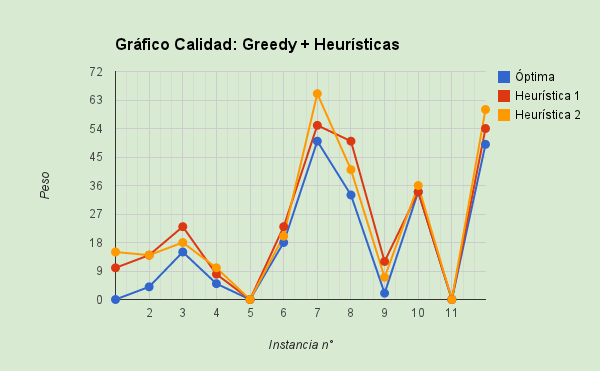
\includegraphics[scale=0.45]{grafico_calicad_greedy_heuristicas.png}

\textbf{En estas condiciones, ninguno es claro vencedor. Esto puede deberse al hecho de que las vecindades son ``similares'' en cuánto a cómo son sus vecinos}, realizar un intercambio de nodos entre 2 conjuntos distintos es lo mismo que tomar un nodo, colocarlo en un conjunto y luego tomar otro nodo distinto y colocarlo en el conjunto donde se encontraba el vértice anteriormente mencionado. 

Lo que si se puede apreciar del gráfico es que las soluciones obtenidas por las heurísticas no son excesivamente lejanas a las óptimas. Dicho fenómeno no ocurre espontáneamente, \textbf{mientras mejor es la solución inical, la solución encontrada por la heurística también lo va a ser.} Formalmente, la respuesta de una heurística, a lo sumo, es igual de buena a la solución inicial, nunca peor, sino caería fuera de la definición de heurística. En consecuencia, tener buenas soluciones iniciales favorece que la heurística acabe en una buena solución final.

\noindent \textbf{Medición de calidad con Solución Aleatoria}

El siguiente gráfico muestra \textbf{instancias sin ningún tipo de particularidad}. La diferencia con el caso anterior es que, inclusive con $k \geq n$, como la solución es generada al azar, no necesariamente la solución obtenida es óptima. Por eso, en estas condiciones, es relevante analizar todos los casos, y no restringirlo a $k < n$.

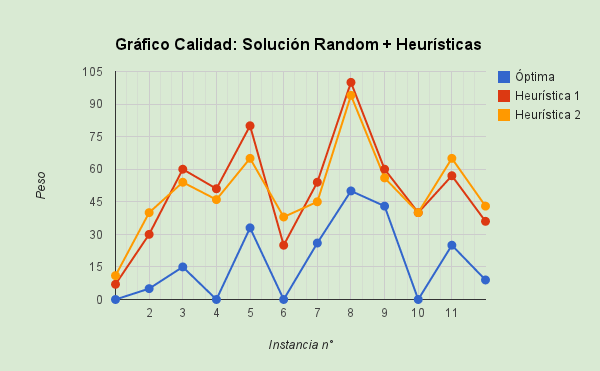
\includegraphics[scale=0.45]{grafico_calicad_greedy_random.png}

Como en el análisis de calidad anterior, \textbf{ninguno de los 2 se destaca claramente.} Por otra parte, es claro que \textbf{las heurísticas entregaron soluciones peores que las del análisis previo}. Las soluciones aleatorias pueden ser excesivamente malas, inclusives las peores, y eso se ve reflejado en los resultados obtenidos. Es fácil ver que, para estas heurísticas, \textbf{siempre conviene tener inicialmente una solución púlida.} Por esto es que, en la introducción a esta sección del trabajo práctico, mencionamos que las \textbf{heurísticas de búsqueda local brindan un servicio de complemento a otros algoritmos, incluyendo heurísticas, de generación de soluciones.} 
\newpage

\noindent \textbf{\underline{Análisis de Tiempos}}

\noindent \textbf{Metodología de medición}

Para cada tamaño n, generamos 100 instancias. Luego, para cada instancia, medimos su tiempo de ejecución 50 veces, quedándonos con la ejecución que menor tiempo tomo. Finalmente, obtuvimos un promedio de esos valores y el resultado de dicha operación es la que fue colocada en los gráficos. Tomamos el mínimo de cada instancia debido a que el procesador atiende varios procesos en simultáneo y, por ende, es díficil obtener un valor fiel de cuánto realmente toma ejecutar el algoritmo sobre la instancia actual. Tomando el mínimo eliminamos la mayor cantidad de tiempo gastado en operaciones fuera de la ejecución de nuestro algoritmo.

\noindent \textbf{Medición de tiempos}

Ya que ambos algoritmos dependen, en cuánto a complejidad temporal, de $k$, una variable que no tiene relación directa con el tamaño de la entrada $n$, decidimos realizar un análisis de tiempos variando el $k$, esto fue lo que obtuvimos:

\begin{figure}[h!]
\begin{subfigure}{0.5\textwidth}
	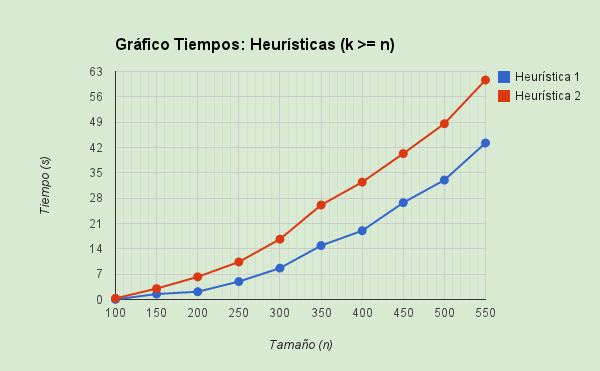
\includegraphics[width=\textwidth, height=60mm]{grafico_tiempos_heuristicas_kmayorigualn.png}
\end{subfigure}
\begin{subfigure}{0.5\textwidth}
	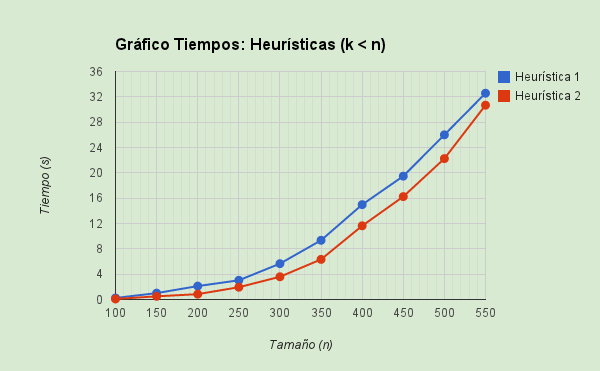
\includegraphics[width=\textwidth, height=60mm]{grafico_tiempos_heuristicas_kmenorn.png}
\end{subfigure}
\end{figure}

\textbf{Los resultados son coherentes al análisis de complejidad hecho anteriormente, el algoritmo 2 está más atado al $k$ que su contraparte}. Pero, conceptualmente, \textbf{¿Cuál es la razón?} Ya habíamos mencionado \textbf{el tamaño de la vecindad de cada heurística: para la 1 el tamaño \boldmath{$\in O(n^2)$} y para la 2da \boldmath{$\in O(n*k)$}}. Si $k < n$, la vecindad de la segunda heurística tiene una cota más ajustada de $O(n^2)$, por eso las mediciones son similares para dicho caso. En cambio, si $k \geq n$, ninguna se tiene una cota mejor. Si bien $O(n^2) = O(n^k)$, para este caso, eso no significa que la vecindad de la heurística 1 depende de $k$, nada más es una cota más ``grosera'' que no refleja el comportamiento adecuadamente. Veamos el siguiente caso: $n = 5$ y $k = 100$, está claro que la vecindad 2 va a ser más numerosa que la 1, independientemente de los pesos de las aristas y de la densidad del grafo. Inclusive, \textbf{uno podría tener un $k$ tan alejado de $n$ como quisiera y así obtener costos temporales potencialmente caros}. 

\textbf{De todas formas, poseemos un algoritmo polinomial que otorga una solución óptima para casos tales que \boldmath{$k \geq n$}} y esa información no es costosa de obtener, se pregunta si eso ocurrre, en $O(1)$, inmediatamente luego de tomar el input. Por lo cuál no habría que preocuparse demasiado por este tipo de casos.

\end{document}
% Fin Ejercicio 1

\newpage
% Comienzo Ejercicio 2
\documentclass[10pt,a4paper]{article}
\usepackage[utf8]{inputenc} % para poder usar tildes en archivos UTF-8
\usepackage[spanish]{babel} % para que comandos como \today den el resultado en castellano
\usepackage{fullpage} %small margins
\usepackage[parfill]{parskip} %genera saltos entre parrafos
\usepackage{color}
\definecolor{gray}{gray}{0.35}
\usepackage{listings}
\usepackage{enumitem}
\usepackage{amsmath} %big brackets
\lstset{
    numbers=left,
    breaklines=true,
    tabsize=2,
    basicstyle=\ttfamily\color{gray},
}
\setlength{\parindent}{8pt}
\usepackage{mathtools}
\usepackage[margin=50pt]{geometry}
\usepackage{amsfonts}
\usepackage{flafter}
\usepackage{multicol}

\begin{document}

\section{Metahurística GRASP}
\subsection{Introduccion}
El problema de K-PMP es un problema muy dificil de resolver, debido a que es NP-Completo le toma mucho tiempo a un algoritmo exacto resolverlo, se puede ver facilmente que para generar todas las particiones posibles, esto no es polinomial (ver ejercicio 2). 

\bigskip
Utilizando una \textit{heuristica constructiva golosa}, se lo pudo resolver en tiempo polinomial aunque obteniendo en su mayor parte soluciones suboptimas  (ver ejercicio 3).

\bigskip
Utilizando una \textit{heuristica de busqueda local}, se pudieron proponer diferentes vecindades para soluciones, este algoritmo de busqueda local es capaz de devolvernos la mejor distribucion de una vecindad dada su solucion, esto es polinomial, pero aun estamos lejos de obtener el valor exacto (ver ejercicio 4).

\bigskip
Lo que se nota utilizando cualquiera de las dos heuristicas anteriormente planteadas entonces es, estamos realizando diferentes estrategias y criterios para tratar de resolver el mismo problema, \textit{mejorando en complejidad temporal pero siempre  sacrificando presicion de la solucion} al problema propiamente dicho.

\bigskip
El objetivo ahora es encontrar una manera de combinar ambas heuristicas, y eventualmente poder llegar a la solucion optima, o al menos poder acercarlo lo suficientemente, sin tener que sacrificar tanto tiempo para su resolucion: La \textbf{Metahuristica GRASP (Greedy Randomized Adaptive Search Procedures)} cumple efectivamente.

\bigskip
Feo y Resende explican como la efectividad de la busqueda local depende de varios factores: la estructura de la vecindad, la funcion a ser minimizada y la solucion con la que se empieza. Una solucion se dice que esta en la \textit{``cuenca de atraccion"} del optimo global si es que la busqueda local arrancando con dicha solucion, lleva al optimo global.

\subsection{Desarrollo}


Para el criterio de busqueda local, se eligio a la primera (local 1, ejercicio 4) debido a que la segunda tiene una vecindad muy parecida a las desiciones de la heuristica golosa y por lo tanto no mejoraba  la solucion. Ahora lo unico que nos hace falta es diferentes soluciones con las cuales arrancar, e ir probandolas hasta poder dar con alguna que este en la cuenca de atraccion, o al menos se acerque al valor de la solucion optima lo suficientemente sin sacrificar gran cantidad de tiempo.

\bigskip
Utilizar soluciones totalmente aleatorias son de calidad pobre en general, la heuristica golosa produce mejores soluciones que las aleatorias, aunque suboptimas: se elije al elemento mejor posicionado, y se lo agrega a la construccion. Esta heuristica siempre vendria a generar la misma solucion, haciendo que si la solucion final no cae en la cuenca de atraccion, nunca se llegaria al optimo global utilizando la busqueda local.

\bigskip
Nuestra heuristica golosa lo que hace es obtener todos los nodos, calcular su peso asociado si estuviesen todos en un solo conjunto, ordenarlos de mayor peso a menor, y luego iterar sobre este conjunto de nodos siempre sacando al de mayor peso y analizando en que conjunto impactaria menos su peso (para mas detalles revisar ejercicio 3).

\newpage
Procedemos entonces a modificar la heuristica golosa y \textbf{aleatorizarla}, lo que le agrega variacion a la construccion anteriormente planteada. En vez de siempre elegir el nodo de mayor peso usamos los esquemas basados en el \textbf{valor} y en la \textbf{cardinalidad}:

\bigskip
Se elijen aleatoriamente $\beta$\% nodos del total, se los ordena de mayor a menor peso, y de todos estos, se elije aleatoriamente un nodo que este entre los mejores $\alpha$\%.

\begin{lstlisting}
nodo function pickOne(nodos, alpha, beta):

	rcl = vector de nodos
	
	Mientras no se hayan elegido beta% nodos del total:
		nodo = Elegir aleatoriamente un nodo entre 0 y el total
		rcl.agregar(nodo)
	Fin Mientras
	
	Ordenar rcl de mayor a menor peso
	nodo = Elegir aleatoriamente del rcl un nodo entre los %alpha mayores
	Eliminar nodo de nodos
	Retornar nodo
	
Fin
\end{lstlisting}

\bigskip
Ahora que ya tenemos nuestra heuristica golosa aleatorizada y la heuristica local, nuestra metaheuristica grasp va a consistir en una combinacion entre ambos hasta cumplir que la solucion f* no mejore luego de 100 iteraciones o se encuentre alguna con peso 0.

\bigskip
\begin{lstlisting}
f* = MAX_VALUE
Repetir hasta que el criterio de parada este cumpla:

	Generar solucion golosa x con parametros alpha y beta
	Busqueda local de un optimo local x', arrancando desde x
	Si f(x') < f*
		f* = f(x')
		x* = x'
	Fin Si
	
Fin
\end{lstlisting}

Los parametros alpha y beta se decidiran en base a las experimentaciones mas adelante, en las cuales se va a comparar para cada valor elegido la mejora de la solucion. Para mas detalles de implementación, ver el codigo fuente adjunto.
\newpage

\subsection{Experimentacion}
Para la siguiente busqueda de los mejores valores de los parametros, se generaron 100 instancias aleatorias con n = 30, m = 435 (Grafo con 30 nodos completo) y k =10, con aristas con peso entre 0 y 100.
Para cada una de las 100 instancias, el experimento se ejecuto 10 veces, y se tomo su  mejor peso, el cual se sumo al mejor peso obtenido de cada una de las instancias, y se obtuvo un promedio entre todas ellas, es decir, el promedio de los mejores valores de las 100 instancias.

Se diseñó un programa que dado un numero x de instancias, r de repeticiones, n de nodos y k de particiones, genera x instancias aleatorias con grafos completos de n nodos.

Procedemos entonces a buscar los mejores valores para $\alpha$ y $\beta$, fijando las 100 iteraciones del grasp, porque si se toma menos de eso es bastante mas probable de no poder dar con una buena solucion, y ya elegir bastante mas que eso demora mucho mas para la experimentacion. La tabla presentada a continuacion refleja los datos de las experimentaciones, donde el contenido es el peso resultado de cada solucion obtenida.

\bigskip
\noindent 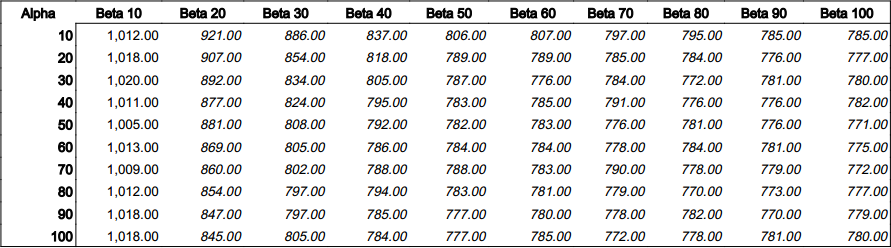
\includegraphics[scale=0.55]{img/values.png} \\
\bigskip
\noindent 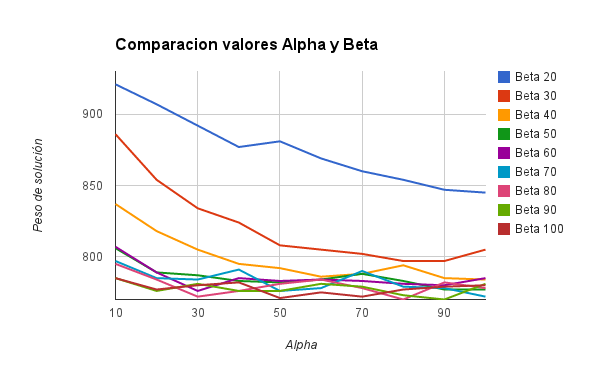
\includegraphics[scale=0.75]{img/grafico_alpha_beta.png} 

El grafico de arriba muestra los datos de la tabla para poder hacer un mejor analisis de los datos obtenidos, debido a que instancias con $\beta$ = 10 generaban soluciones con peso mucho mayor se los excluyo del grafico.

Se puede ver que a partir $\beta$ = 50 las soluciones tienden a tener un mismo peso pero con una leve distorción. Se puede observar que con $\beta$ = 100 se obtienen uno de los mejores resultados aunque revela saltos de vez en cuando. Sin embargo en la tabla de datos, uno de los mejores candidatos para ambos valores son con $\alpha$ = 80 y $\beta$ = 80, mas alla de que esta desición puede no ser la mejor, no esta lejos de serla tampoco, ya que todos los valores alrededor de esa configuracion son bastante menores que los demas.


\end{document}
% Fin Ejercicio 2

%\newpage
% Comienzo Ejercicio 3
%\documentclass[10pt,a4paper]{article}
\usepackage[utf8]{inputenc} % para poder usar tildes en archivos UTF-8
\usepackage[spanish]{babel} % para que comandos como \today den el resultado en castellano
\usepackage{fullpage} %small margins
\usepackage[parfill]{parskip} %genera saltos entre parrafos
\usepackage{color}
\definecolor{gray}{gray}{0.35}
\usepackage{listings}
\usepackage{enumitem}
\usepackage{amsmath} %big brackets
\lstset{
    numbers=left,
    breaklines=true,
    tabsize=2,
    basicstyle=\ttfamily\color{gray},
}
\setlength{\parindent}{8pt}
\usepackage{mathtools}
\usepackage[margin=50pt]{geometry}
\usepackage{amsfonts}
\usepackage{flafter}
\usepackage{multicol}

\begin{document}

\section{Experimentación sobre cada heurística implementada}
\end{document}
% Fin Ejercicio 3

\end{document}